\documentclass[9pt]{beamer}

\usepackage[utf8x]{inputenc}
\usepackage{MinionPro}
\usefonttheme{serif} 
\usepackage{xspace}
\usepackage{tikz}
\usepackage{listings}
\usepackage[vlined,linesnumbered]{algorithm2e}
\usepackage{comment}

\definecolor{oxygenorange}{HTML}{FF7522}



\mode<presentation>
{
  \setbeamercovered{transparent}
  \setbeamercolor{normal text}{fg=white,bg=gray}
  \setbeamercolor{alerted text}{fg=white}
  \setbeamercolor{example text}{fg=white}
  \setbeamercolor{background canvas}{bg=darkgray} 
  \setbeamercolor{structure}{fg=white}

  \setbeamercolor{block title}{bg=oxygenorange,fg=white}
  \setbeamercolor{block body}{bg=white,fg=darkgray}

  \setbeamercolor{palette primary}{use=structure,fg=structure.fg}

  \setbeamercolor{math text}{}
  \setbeamercolor{math text inlined}{parent=math text}
  \setbeamercolor{math text displayed}{parent=math text}

  \setbeamercolor{normal text in math text}{}

  \setbeamercolor{local structure}{parent=structure}

  \setbeamercolor{titlelike}{parent=structure}

  \setbeamercolor{title}{parent=titlelike}
  \setbeamercolor{title in head/foot}{parent=palette quaternary}
  \setbeamercolor{title in sidebar}{parent=palette sidebar quaternary}

  \setbeamercolor{subtitle}{parent=title}
}

\renewcommand{\emph}[1]{\textbf{\color{oxygenorange}#1}\xspace}
\newcommand{\field}[1]{\ensuremath{\mathbb{#1}}}
\newcommand{\F}{\ensuremath{\field{F}}}
% \newcommand{\PolyBoRi}{\textsc{PolyBoRi}\xspace}
% \newcommand{\Magma}{\textsc{Magma}\xspace}
% \newcommand{\Singular}{\textsc{Singular}\xspace}
\newcommand{\E}{\ensuremath{\textnormal{E}}}
\newcommand{\Var}{\ensuremath{\textnormal{Var}}}
\DeclareMathOperator{\erf}{erf}

\newcommand{\patchit}[1]{\begin{block}{send us a patch}#1\end{block}}
\newcommand{\PRESENT}{\textsc{Present}\xspace}
\newcommand{\M}[1]{\ensuremath{\textsc{M}(#1)\xspace}}
\newcommand{\LT}[1]{\ensuremath{\textsc{LT}(#1)\xspace}}
\newcommand{\LM}[1]{\ensuremath{\textsc{LM}(#1)\xspace}}
\newcommand{\LC}[1]{\ensuremath{\textsc{LC}(#1)\xspace}}
\newcommand{\LCM}[1]{\ensuremath{\textsc{LCM}(#1)\xspace}}
\newcommand{\ideal}[1]{\langle #1 \rangle}

\lstdefinelanguage{Sage}[]{Python}{morekeywords={True,False,sage,cdef,cpdef,ctypedef,self},sensitive=true}
\lstset{frame=none,
          showtabs=False,
          showspaces=False,
          showstringspaces=False,
          commentstyle={\color{oxygenorange}},
          keywordstyle={\color{lightgray}},
          stringstyle ={\color{lightgray}},
          language = Sage,
          basicstyle=\footnotesize\tt
          }


\title{Sage \& Algebraic Techniques for the Lazy Symmetric Cryptographer}
\author{Martin R.\ Albrecht\\{@martinralbrecht}}
\institute{Crypto Group, DTU Compute, Denmark}
\date{IceBreak, Reykjavik, Iceland\\{\#icebreak}}

\AtBeginSubsection[] {
   \begin{frame}{Outline}
  \tableofcontents[currentsubsection]
  \end{frame}
}


\begin{document}

\begin{frame}
\titlepage
\end{frame}

\begin{frame}{Outline}
\tableofcontents
\end{frame}

\section{Sage}

\subsection{Introduction}

\begin{frame}
\frametitle{Blurb}

\begin{columns}

\column{0.15\textwidth}

\begin{center}
 
\includegraphics[height=0.9\textwidth]{./sage-logo.png}
\vspace{0.5em}
\end{center}

\column{0.8\textwidth}
\begin{block}{Sage open-source mathematical software system}
``Creating a viable free open source alternative to Magma, Maple, Mathematica and Matlab.''
\end{block}
\end{columns}

\vspace{1em}

Sage is a free open-source mathematics software system licensed under the GPL. It combines the power of many existing open-source packages into a common Python-based interface.

\vspace{1em}

\begin{tabular}{ll}
First release 2005 & Latest version 5.9 released 2013-05-03\\
$>$ 300 releases  & Shell, webbrowser (GUI), library\\
$>$ 180 developers  & $\sim 100$ components\\
$>$ 200 papers cite Sage & $> 2100$ subscribers [sage-support]\\
$>$ 100,000 web visitors/month&  $> 6,500$ downloads/month\\
\end{tabular}
\end{frame}

\begin{frame}
\frametitle{How to use it}
Sage can be used via the command line, as a webapp hosted on your local computer and via the Internet, or embedded on any website.

\begin{center}
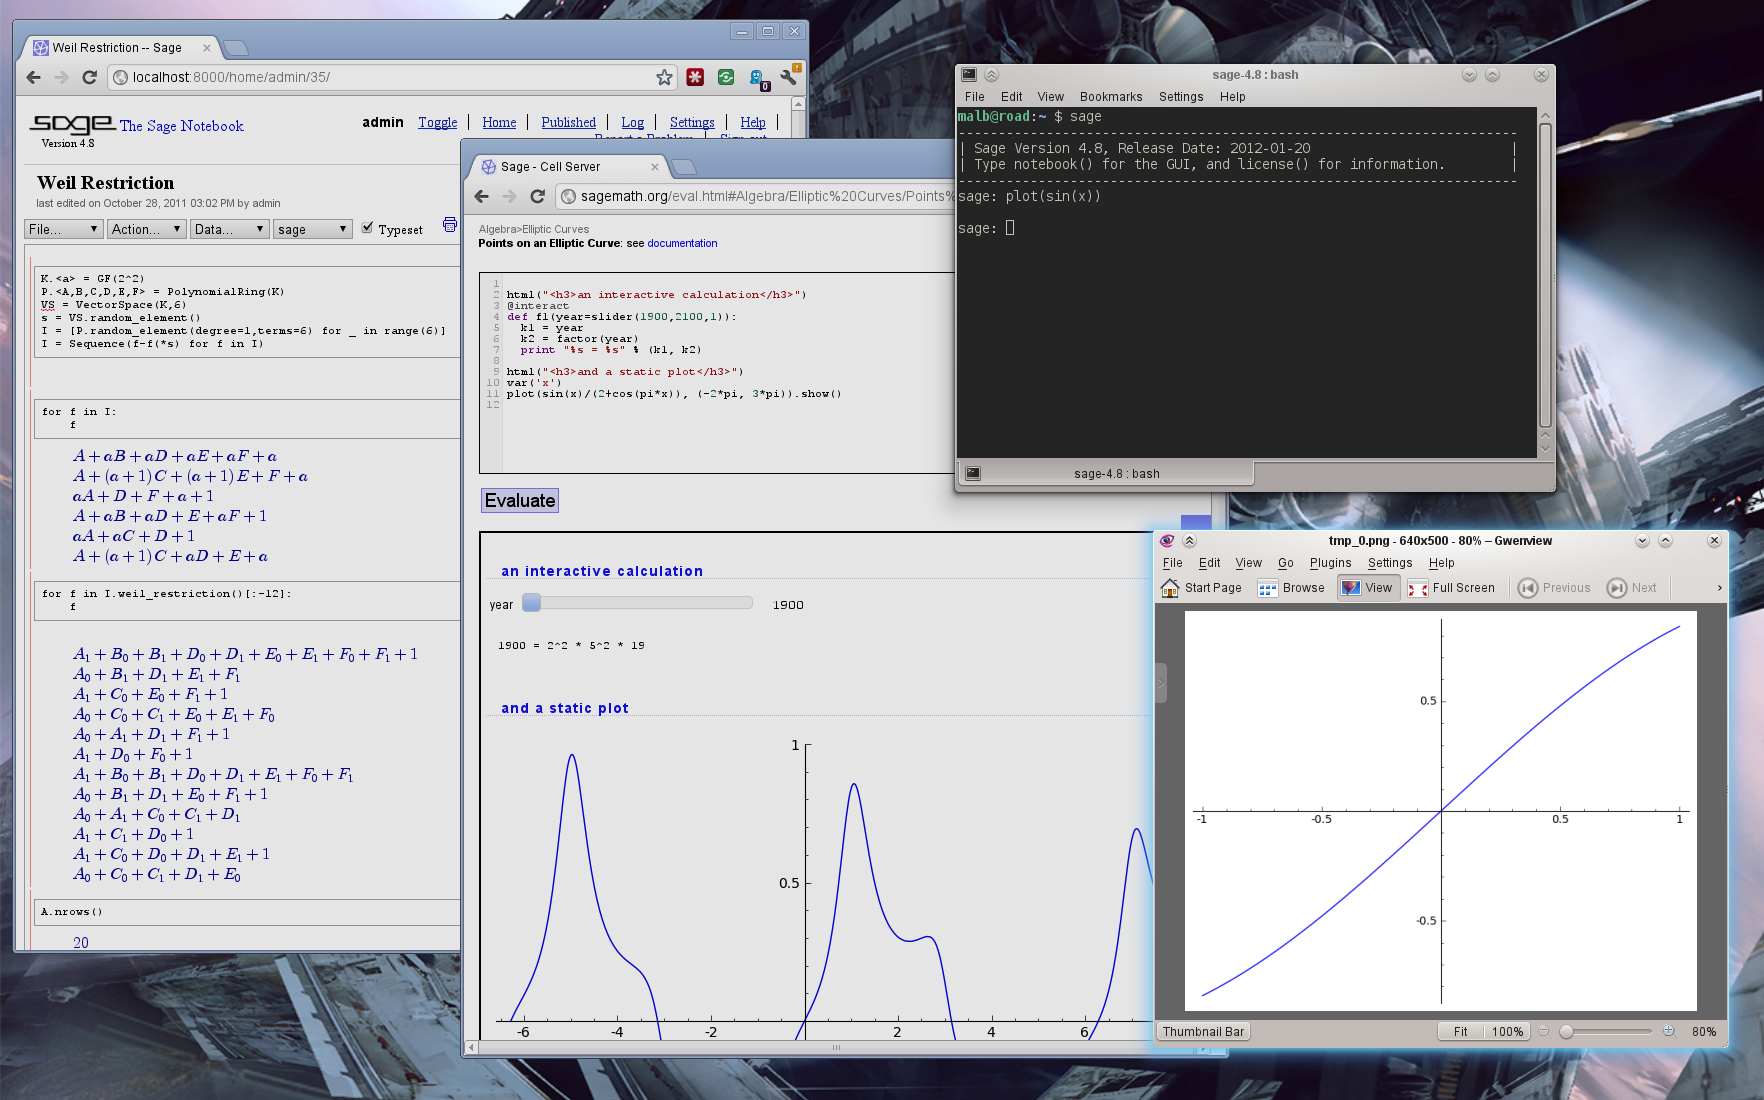
\includegraphics[width=0.7\textwidth]{sage-desktop.png}
\end{center}
\vspace{-0.5em}
\begin{block}{}
Check out: \url{http://aleph.sagemath.org} and \url{https://cloud.sagemath.com/}
\end{block}
\end{frame}

\begin{frame}
\frametitle{``How do I do \dots in Sage?''}
\framesubtitle{\hfill \dots It's easy: implement it and send us a patch.}

Sage is a largely volunteer-driven effort, this means that
\begin{itemize}
 \item developers work on whatever suits their needs best;
 \item the quality of code in Sage varies:
 \begin{itemize}
   \item is a generic or a specialised, optimised implementation used,
   \item how much attention is paid to details,
   \item is your application an untested ``corner case'',
   \item how extensive are the tests, the documentation, or
   \item is the version of a particular package up to date.
 \end{itemize}
 \item you cannot expect people to fix your favourite bug quickly (although we do try!),
 \item you can get involved and make Sage better for your needs!
\end{itemize}

\patchit{I will highlight relevant issues to encourage you to get involved.}
\end{frame}

\subsection{Highlevel Features}

\begin{frame}[fragile]
\frametitle{Python \& Cython}
\begin{block}{}
\centering
 
\includegraphics[width=0.4\textwidth]{python-and-cython.png}
\end{block}

Sage does \emph{not} come with yet-another ad-hoc mathematical programming language, it uses
\emph{Python} instead.

\begin{itemize}
\item one of the most widely used programming languages (Google, IML, YouTube, NASA),
\item easy for you to define your own data types and methods on it (bitstreams, ciphers, rings, whatever),
\item very clean language that results in easy to read code,
\item a \emph{huge number of libraries}: statistics, networking, databases,
bioinformatic, physics, video games, 3d graphics, numerical computation (scipy),
and serious ``pure'' mathematics (via Sage)
\item easy to use existing C/C++ libraries from Python (via \emph{Cython})
\end{itemize}
\end{frame}



% \begin{frame}[fragile]
% \frametitle{Python Example: Databases}
% 
% \begin{lstlisting}
% sage: import sqlalchemy as S
% sage: db = S.create_engine('sqlite:///tutorial.db')
% sage: users = S.Table('users', S.MetaData(db),
%               S.Column('user_id', S.Integer, primary_key=True),
%               S.Column('name', S.String(40r)),
%               S.Column('modulus', S.String)).create()
% 
% sage: i = users.insert()
% sage: M = random_prime(2^512)*random_prime(2^512)
% sage: i.execute(name='Mary',modulus=str(M))
% 
% sage: s = users.select(whereclause="name='Mary'")
% sage: row = s.execute().fetchone()
% sage: ZZ(row[users.c.modulus])
% 56974631402866323...250077669
% \end{lstlisting}
% 
% \end{frame}

\begin{frame}[fragile]
\frametitle{Python Example: Networking}
\begin{small}
\emph{Scapy} is a powerful interactive packet manipulation program written in Python. It is able to forge or decode packets of a wide number of protocols, send them on the wire, capture them, match requests and replies, and much more. It can easily handle most classical tasks like scanning, tracerouting, probing, unit tests, attacks or network discovery.
\end{small}

\begin{lstlisting}
from scapy.all import *

class Test(Packet):
    name = "Test packet"
    fields_desc = [ ShortField("test1", 1),
                    ShortField("test2", 2) ]

print Ether()/IP()/Test(test1=x,test2=y)

p=sr1(IP(dst="127.0.0.1")/ICMP())
if p:
    p.show()
\end{lstlisting}
\end{frame}

\begin{frame}[fragile]
\frametitle{Cython: Your Own Code}
\begin{lstlisting}
sage: cython("""
def foo(unsigned long a, unsigned long b):
  cdef int i
  for i in range(64):
    a ^= a*(b<<i)
  return a
""")
sage: foo(a,b)
\end{lstlisting}

\vspace{1em}

This generates C code like this:

\begin{lstlisting}[language=c]
for (__pyx_t_1 = 0; __pyx_t_1 < 64; __pyx_t_1+=1) {
    __pyx_v_i = __pyx_t_1;
    __pyx_v_a = (__pyx_v_a ^ _pyx_v_a * (__pyx_v_b << __pyx_v_i));
}
\end{lstlisting}
\end{frame}

\begin{frame}[fragile,allowframebreaks]
\frametitle{Cython: External Code}
\begin{lstlisting}
#cargs -std=c99 -ggdb
cdef extern from "katan.c":
    ctypedef unsigned long uint64_t
    void katan32_encrypt(uint64_t *p, uint64_t *c, uint64_t *k, int nr)
    void katan32_keyschedule(uint64_t *k, uint64_t *key, int br)
    uint64_t ONES

def k32_encrypt(plain, key):
    cdef int i
    cdef uint64_t _plain[32], _cipher[32], kk[2*254], _key[80]

    for i in range(80):
        _key[i] = ONES if key[i] else 0
    for i in range(32):
        _plain[i] = ONES if plain[i] else 0

    katan32_keyschedule(kk, _key, 254)
    katan32_encrypt(_plain, _cipher, _key, 254)

    return [int(_cipher[i]%2) for i in range(32)]

sage: load("sage-katan.spyx")
sage: k32_encrypt(random_vector(GF(2),32),random_vector(GF(2),80))
[1, 0, 0, 1, 0, 1, 0, 0, 0, 1, ... 0, 1, 0, 0]
\end{lstlisting}

\framebreak


\begin{lstlisting}
sage: rv = lambda : random_vector(GF(2),32)
sage: E = lambda : k32_encrypt(rv(),rv())

sage: l = [E() for _ in range(1024)]
sage: l = [sum(e) for e in l]
sage: r.summary(l) # We are using R!
Min. 1st Qu.  Median    Mean 3rd Qu.    Max.
8.00   14.00   16.00   16.03   18.00   27.00

sage: c = E()
sage: K = GF(next_prime(2^32))
sage: g = K(sum(2^i*c[i] for i in range(32))); g
2859908881
sage: g.multiplicative_order() # We are using Pari/GP
858993462

sage: A = matrix(GF(2),32,32,[E() for _ in range(32)])
sage: A.rank() # We are using M4RI
30
\end{lstlisting}


\end{frame}


\begin{frame}[fragile]
\frametitle{Symmetric Multiprocessing}

Embarrassingly parallel computations on multicore machines are easy in Sage:

\begin{lstlisting}
sage: @parallel(2)
....: def f(n):
....:     return factor(n)
....:

sage: %time _ = [f(2^217-1), f(2^217-1)]
CPU times: user 1.07 s, sys: 0.02 s, total: 1.09 s
Wall time: 1.10 s

sage: %time _ = list( f([2^217-1, 2^217-1]) )
CPU times: user 0.00 s, sys: 0.02 s, total: 0.02 s
Wall time: 0.62 s

sage: 1.08/0.62
1.74193548387097
\end{lstlisting}
\end{frame}

\subsection{Fields \& Areas}

\begin{frame}[fragile]
\frametitle{Dense Linear Algebra}

\begin{lstlisting}
sage: for p in (2,3,4,5,7,8,9,11):
....:     K = GF(p,'a')
....:     A = random_matrix(K,2000,2000)
....:     B = random_matrix(K,2000,2000)
....:     t = cputime()
....:     C = A*B
....:     print "%32s %7.3f"%(K,cputime(t))
....:
Finite Field of size 2          0.008 # M4RI
Finite Field of size 3          0.972 # LinBox
Finite Field in a of size 2^2   0.048 # M4RIE
Finite Field of size 5          0.996 # LinBox
Finite Field of size 7          0.968 # LinBox
Finite Field in a of size 2^3   0.072 # M4RIE
Finite Field in a of size 3^2 695.863 # generic
Finite Field of size 11         1.020 # LinBox
\end{lstlisting}

\patchit{We know how to make $\F_{p^k}$ really fast, but someone needs to step up.\\
{\tt FLINT} 2.3 (in Sage 5.10) improves $\F_p$ for $2^{23} < p<2^{64}$, but an interface is missing.}

\end{frame}

\begin{frame}[fragile]
\frametitle{Sparse Linear Algebra}

to construct and compute with sparse matrices by using the {\tt sparse=True} keyword.

\begin{lstlisting}
sage: A = random_matrix(GF(32003),2000,2000,density=~200,sparse=True)
sage: %time copy(A).rank() # LinBox
CPU times: user 3.26 s, sys: 0.05 s, total: 3.31 s
Wall time: 3.33 s
2000
sage: %time copy(A).echelonize() # custom code
CPU times: user 9.51 s, sys: 0.02 s, total: 9.52 s
Wall time: 9.56 s
sage: v = random_vector(GF(32003),2000)
sage: %time _ = copy(A).solve_right(v) # LinBox + custom code
CPU times: user 3.74 s, sys: 0.00 s, total: 3.74 s
Wall time: 3.76 s
\end{lstlisting}

\patchit{\texttt{LinBox}'s claim to fame is good support for \emph{black box} algorithms for sparse and structured matrices. Help us to expose more of this functionality.}
\end{frame}

\begin{frame}[fragile]
\frametitle{Lattices}
Sage includes both \texttt{NTL} and \texttt{fpLLL}:

\begin{lstlisting}
sage: from sage.libs.fplll.fplll import gen_intrel  # Knapsack-style
sage: A = gen_intrel(50,50); A
50 x 51 dense matrix over Integer Ring ...
sage: min(v.norm().n() for v in A.rows())
2.17859318110950e13

sage: L = A.LLL() # using fpLLL, NTL optional
sage: L[0].norm().n()
5.47722557505166

sage: L = A.BKZ() # using NTL
sage: L[0].norm().n()
3.60555127546399
\end{lstlisting}

\patchit{Our version of \texttt{fpLLL} is old (to be updated in 5.11, but an interface to its BKZ is missing).}


\end{frame}

\begin{frame}[fragile]
\frametitle{Symbolics}
Sage uses {\tt Pynac} ({\tt GiNaC} fork) and {\tt Maxima} for most of its symbolic manipulation. {\tt SymPy} is included in Sage as well.

\begin{lstlisting}
sage: q = var('q')
sage: expr = (1-1/q)/(q-1)
sage: f = expr.function(q); f
q |--> -(1/q - 1)/(q - 1)
sage: f(10)
1/10
sage: f(q^2)
-(1/q^2 - 1)/(q^2 - 1)
sage: f(0.1)
10.0000000000000
sage: g = P.random_element(); g
4*x^2 + 3/4*x
sage: f(g)
-4*(4/((16*x + 3)*x) - 1)/((16*x + 3)*x - 4)

sage: expr.simplify_full()
1/q
sage: expr.integrate(q)
log(q)
\end{lstlisting}
\end{frame}


\begin{frame}[fragile]
\frametitle{Statistics}
Sage ships {\tt R} which is a very powerful package for doing statistics, Sage also uses {\tt SciPy} for stats related tasks.

\begin{lstlisting}
sage: O() # some oracle
sage: l = [O() for _ in range(10000)] # we sample it
sage: r.summary(l) # and ask R about it
  Min.  1st Qu.   Median     Mean  3rd Qu.     Max.
-154.000  -31.000    2.000    0.298   33.000  140.000
sage: import pylab # use pylab to compute a histogram
sage: a,b,_ = pylab.hist(l,100)
sage: line(zip(b,a)) # and Sage's code to plot it
\end{lstlisting}

\begin{columns}
\column{0.5\textwidth}
\centering
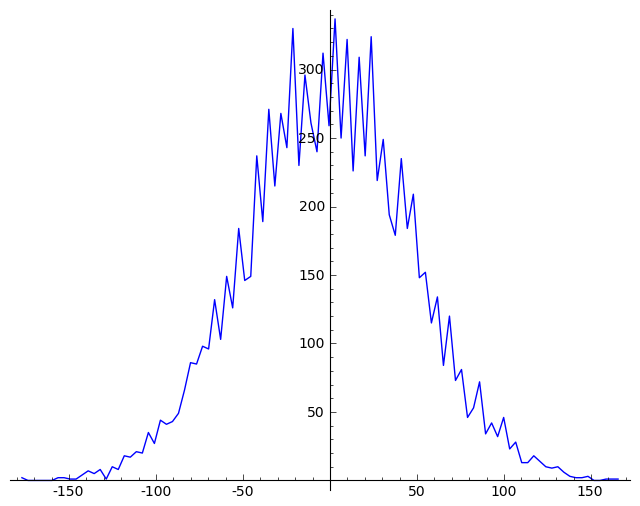
\includegraphics[width=0.7\textwidth]{gaussian.png}
\column{0.5\textwidth}
\patchit{Our interface to R could be greatly improved}
\end{columns}
\end{frame}


\begin{frame}[fragile]
\frametitle{Coding Theory}
Computations in coding theory are mainly realised by GAP. For example, we can ask about the minimum distance of a code.

\begin{lstlisting}
sage: A = random_matrix(GF(2), 8, 8)
sage: while A.rank() != 8: A = random_matrix(GF(2), 8, 8)
sage: A
[0 0 0 0 1 0 1 0]
[1 1 0 1 1 1 1 0]
[0 0 1 1 0 1 1 0]
[0 0 0 1 0 1 1 0]
[0 0 0 0 0 0 1 0]
[0 1 0 1 0 0 1 0]
[1 0 1 0 1 0 0 1]
[1 0 0 1 1 1 0 0]
sage: G = matrix(GF(2), 8, 8, 1).augment(A.T)
sage: LinearCodeFromCheckMatrix(G).minimum_distance()
\end{lstlisting}

\patchit{Our interface to GAP sucks, try doing the same over $\F_{2^e}$ to see how much.\\Our coding theory is rather basic: things tend to get pushed down to linear codes, i.e., disregarding their structure.}
\end{frame}

\begin{frame}[fragile]
\frametitle{Graph Theory}
\begin{itemize}
\item builds on {\tt NetworkX} (Los Alamos's Python graph library)
\item graph isomorphism testing -- Robert Miller's new implementation
\item graph databases
\item 2d and 3d visualization
\end{itemize}
\begin{lstlisting}
sage: D = graphs.DodecahedralGraph()
sage: D.show3d()
\end{lstlisting}
\vspace{-5em}
\begin{flushright}
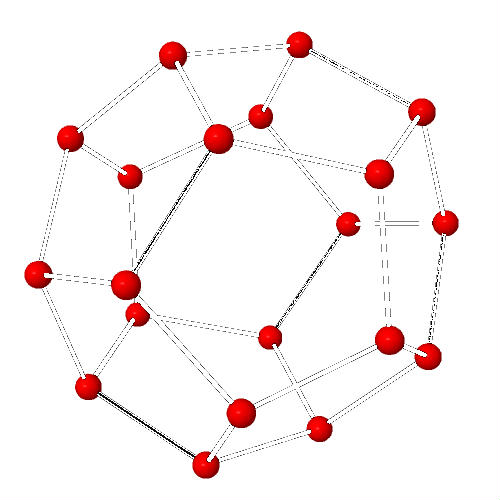
\includegraphics[width=0.3\textwidth]{graph3d.jpeg}
\end{flushright}
\vspace{-2em}
\begin{lstlisting}
sage: E = D.copy()
sage: gamma = SymmetricGroup(20).random_element()
sage: E.relabel(gamma)
sage: D.is_isomorphic(E)
True
sage: D.radius()
5
\end{lstlisting}
\end{frame}

\begin{frame}[fragile,allowframebreaks]
\frametitle{S-Boxes}

\begin{itemize}
 \item We create the \PRESENT S-box
\begin{lstlisting}
sage: S = mq.SBox(12,5,6,11,9,0,10,13,3,14,15,8,4,7,1,2); S
(12, 5, 6, 11, 9, 0, 10, 13, 3, 14, 15, 8, 4, 7, 1, 2)
sage: type(S)
<class 'sage.crypto.mq.sbox.SBox'>
\end{lstlisting}
 \item evaluate it
\begin{lstlisting}
sage: S(0)
12
sage: S([0,0,0,1])
[0, 1, 0, 1]
\end{lstlisting}
\item compute the interpolation polynomial
\begin{lstlisting}
sage: f = S.interpolation_polynomial()
sage: f(0), S(0)
(a^3 + a^2, 12)
\end{lstlisting}
\begin{eqnarray*}
f &=& a^{13}(x^{14} + x^{13}) + a^{6}(x^{12} + x^{6} + 1) +  a^{11}(x^{11} + x^4) + a^{14}(x^{10} + x^{9}) + \\
 & &  a^{10}(x^{8} + x^{3} + x^{2}) + a^{2}x^{7} + a^{9}x^{5}
\end{eqnarray*}

\framebreak

\item compute the linear approximation matrix
\begin{lstlisting}
sage: S = mq.SBox(12,5,6,11,9,0,10,13,3,14,15,8,4,7,1,2)
sage: S.linear_approximation_matrix()
[ 8  0  0  0  0  0  0  0  0  0  0  0  0  0  0  0]
[ 0  0  0  0  0 -4  0 -4  0  0  0  0  0 -4  0  4]
[ 0  0  2  2 -2 -2  0  0  2 -2  0  4  0  4 -2  2]
[ 0  0  2  2  2 -2 -4  0 -2  2 -4  0  0  0 -2 -2]
[ 0  0 -2  2 -2 -2  0  4 -2 -2  0 -4  0  0 -2  2]
[ 0  0 -2  2 -2  2  0  0  2  2 -4  0  4  0  2  2]
[ 0  0  0 -4  0  0 -4  0  0 -4  0  0  4  0  0  0]
[ 0  0  0  4  4  0  0  0  0 -4  0  0  0  0  4  0]
[ 0  0  2 -2  0  0 -2  2 -2  2  0  0 -2  2  4  4]
[ 0  4 -2 -2  0  0  2 -2 -2 -2 -4  0 -2  2  0  0]
[ 0  0  4  0  2  2  2 -2  0  0  0 -4  2  2 -2  2]
[ 0 -4  0  0 -2 -2  2 -2 -4  0  0  0  2  2  2 -2]
[ 0  0  0  0 -2 -2 -2 -2  4  0  0 -4 -2  2  2 -2]
[ 0  4  4  0 -2 -2  2  2  0  0  0  0  2 -2  2 -2]
[ 0  0  2  2 -4  4 -2 -2 -2 -2  0  0 -2 -2  0  0]
[ 0  4 -2  2  0  0 -2 -2 -2  2  4  0  2  2  0  0]
\end{lstlisting}

\framebreak

\item and the difference distribution matrix:
\begin{lstlisting}
sage: S = mq.SBox(12,5,6,11,9,0,10,13,3,14,15,8,4,7,1,2)
sage: S.difference_distribution_matrix()
[16  0  0  0  0  0  0  0  0  0  0  0  0  0  0  0]
[ 0  0  0  4  0  0  0  4  0  4  0  0  0  4  0  0]
[ 0  0  0  2  0  4  2  0  0  0  2  0  2  2  2  0]
[ 0  2  0  2  2  0  4  2  0  0  2  2  0  0  0  0]
[ 0  0  0  0  0  4  2  2  0  2  2  0  2  0  2  0]
[ 0  2  0  0  2  0  0  0  0  2  2  2  4  2  0  0]
[ 0  0  2  0  0  0  2  0  2  0  0  4  2  0  0  4]
[ 0  4  2  0  0  0  2  0  2  0  0  0  2  0  0  4]
[ 0  0  0  2  0  0  0  2  0  2  0  4  0  2  0  4]
[ 0  0  2  0  4  0  2  0  2  0  0  0  2  0  4  0]
[ 0  0  2  2  0  4  0  0  2  0  2  0  0  2  2  0]
[ 0  2  0  0  2  0  0  0  4  2  2  2  0  2  0  0]
[ 0  0  2  0  0  4  0  2  2  2  2  0  0  0  2  0]
[ 0  2  4  2  2  0  0  2  0  0  2  2  0  0  0  0]
[ 0  0  2  2  0  0  2  2  2  2  0  0  2  2  0  0]
[ 0  4  0  0  4  0  0  0  0  0  0  0  0  0  4  4]
\end{lstlisting}
\framebreak

\item recover a bunch of boolean polynomials that satisfy the relations of the S-box:
\begin{lstlisting}
sage: S = mq.SBox(12,5,6,11,9,0,10,13,3,14,15,8,4,7,1,2)
sage: S.polynomials() #default: degree=2
[x1*x2 + x0 + x1 + x3 + y3,
 x0*x1 + x0*x2 + x0 + x1 + y0 + y2 + y3 + 1,
 x0*x3 + x1*x3 + x1*y0 + x0*y1 + x0*y2 + x1 + x2 + y2,
 x0*x3 + x0*y0 + x1*y1 + x0 + x2 + y2,
 x0*x2 + x0*y0 + x0*y1 + x1*y2 + x1 + x2 + x3 + y2 + y3, ...]
\end{lstlisting}

\item write the S-box in algebraic normal form
\begin{lstlisting}
sage: S = mq.SBox(12,5,6,11,9,0,10,13,3,14,15,8,4,7,1,2)
sage: P.<y0,y1,y2,y3,x0,x1,x2,x3> = PolynomialRing(GF(2),order='lex')
sage: X = [x0,x1,x2,x3]
sage: Y = [y0,y1,y2,y3]
sage: S.polynomials(X=X,Y=Y,degree=3,groebner=True)
[y0 + x0*x1*x3 + x0*x2*x3 + x0 + x1*x2*x3 + x1*x2 + x2 + x3 + 1,
 y1 + x0*x1*x3 + x0*x2*x3 + x0*x2 + x0*x3 + x0 + x1 + x2*x3 + 1,
 y2 + x0*x1*x3 + x0*x1 + x0*x2*x3 + x0*x2 + x0 + x1*x2*x3 + x2,
 y3 + x0 + x1*x2 + x1 + x3]
\end{lstlisting}
\end{itemize}

\end{frame}

\begin{frame}[fragile,allowframebreaks]
\frametitle{Boolean Functions}


\begin{lstlisting}
sage: from sage.crypto.boolean_function import *
sage: P.<x0,x1,x2,x3> = BooleanPolynomialRing()
sage: b = x0*x1 + x2*x3
sage: f = BooleanFunction(b)
sage: [b(x[0],x[1],x[2],x[3]) for x in GF(2)^4]
[0, 0, 0, 1, 0, 0, 0, 1, 0, 0, 0, 1, 1, 1, 1, 0]
sage: f.truth_table()
(False, False, False, True, False, False, False, True, False, False,
 False, True, True, True, True, False)
\end{lstlisting}

\framebreak

\begin{lstlisting}
sage: WT = f.walsh_hadamard_transform(); WT
(-4, -4, -4, 4, -4, -4, -4, 4, -4, -4, -4, 4, 4, 4, 4, -4)
sage: f.absolute_walsh_spectrum()
{4: 16}
sage: f.nonlinearity()
6
sage: 2^(4-1) - (1/2)*max([abs(x) for x in WT])
6
\end{lstlisting}

\framebreak

\begin{lstlisting}
sage: f.autocorrelation()
(16, 0, 0, 0, 0, 0, 0, 0, 0, 0, 0, 0, 0, 0, 0, 0)
sage: f.absolute_autocorrelation()
{16: 1, 0: 15}
sage: f.absolut_indicator()
0
sage: f.is_bent()
True
sage: f.is_balanced()
False
sage: f.is_symmetric()
False
sage: f.sum_of_square_indicator()
256
sage: f.correlation_immunity()
0
\end{lstlisting}

\begin{lstlisting}
sage: R.<x> = GF(2^8,'a')[]
sage: B = BooleanFunction(x^31)
sage: B.algebraic_immunity()
4
\end{lstlisting}
\end{frame}

\section{Algebraic Techniques}

\subsection{Introduction}

\begin{frame}{Here's a picture of a kitten}
\begin{center}
 
\includegraphics[width=0.9\textwidth]{./kitten-01.jpg}
 % kitten-01.jpg: 1280x800 pixel, 72dpi, 45.16x28.22 cm, bb=0 0 1280 800
\end{center}
 
\end{frame}

\begin{frame}
\frametitle{What are Algebraic Attacks?} 

\begin{enumerate}
 \item Algebraic attacks model a cryptographic primitive (such as a block cipher) as a system of equations.
 \item Then, by applying (algebraic) transformations to these equations they (attempt to) recover information about the secret of the primitive (the key).
\end{enumerate}

\begin{block}{}
Hence, they are quite different in spirit from statistical techniques such as linear and differential cryptanalysis.
\end{block}

\end{frame}


\begin{frame}
\frametitle{A Polemic History of Algebraic Attacks I}
\textbf{1959} -- the ``prophecy''\footnote{This quote is often given to back up the claim that Claude Shannon predicted algebraic attacks. I don't think this quote delivers this. It merely states a design goal not that different from what is now known as provable security.}
\begin{quote}
``Thus, if we could show that solving a certain system requires at least as much work as solving a system of
simultaneous equations in a large number of unknowns, of a complex type, then we would have a lower bound of sorts for
the work characteristic.'' 
\end{quote}
\begin{flushright}
\vspace{-2em}
-- Claude Shannon
\end{flushright}
\end{frame}

\begin{frame}
\frametitle{A Polemic History of Algebraic Attacks II}

\textbf{2002} -- the breakthrough
\begin{quote}
Crucial Cipher Flawed, Cryptographers Claim -- Two cryptographers say that the new Advanced Encryption Standard, [\dots] has a hole in it. Although some of their colleagues doubt the validity of their analysis, the cryptographic community is on edge, wondering whether the new cipher can withstand a future assault.
\end{quote}
\begin{flushright}
\vspace{-2em}
-- Science Magazine
\end{flushright}

\end{frame}

\begin{frame}
\frametitle{A Polemic History of Algebraic Attacks III}
\textbf{2011} -- the disillusion

\begin{tabular}{ll}
 & \\
\hspace{0.05cm} & No proper \emph{block cipher} has been broken using algebraic techniques\\
 & faster than with other techniques\\
\end{tabular}
\end{frame}

\begin{frame}
\frametitle{So, why bother?}

Algebraic techniques 
\begin{enumerate}
 \item are one of the few choices if very few plaintext-ciphertext pairs are available,
 \item become more relevant as focus shifts toward (very) lightweight constructions,
 \item can be combined with other techniques such as side-channel attacks,
 \item offer a trade-off for researcher time vs.\ CPU times
 \item are fun \dots well, to some anyway!
\end{enumerate}
 
\end{frame}


\subsection{Equations}

\begin{frame}[allowframebreaks]
\frametitle{SP-Networks} 

We construct an equation system for the block cipher \PRESENT, which

\begin{itemize}
 \item is a substituion-permutation network,
 \item has a block size of 64 bits,
 \item either takes 80-bit or 128-bit keys (\PRESENT-80 and -128 resp.)
 \item has 31 rounds (shorter variants are denoted by \PRESENT-\{80,128\}-$Nr$),
 \item is conceptually simple, and
 \item has been extensively studied.
\end{itemize}

\begin{small}
\begin{thebibliography}{present}
\bibitem{present}
A.\ Bogdanov, L.\ Knudsen, G.\ Leander, C.\ Paar, A.\ Poschmann, M.\ Robshaw, Y.\ Seurin, and C.\ Vikkelsoe.
\newblock {PRESENT}: An ultra-lightweight block cipher.
\newblock In {\em Cryptographic Hardware and Embedded Systems - CHES 2007},
  volume 7427 of {\em Lecture Notes in Computer Science}, pages 450--466,
  Berlin, Heidelberg, New York, 2007. Springer Verlag.
\end{thebibliography}
\end{small}
\framebreak

\begin{center}
 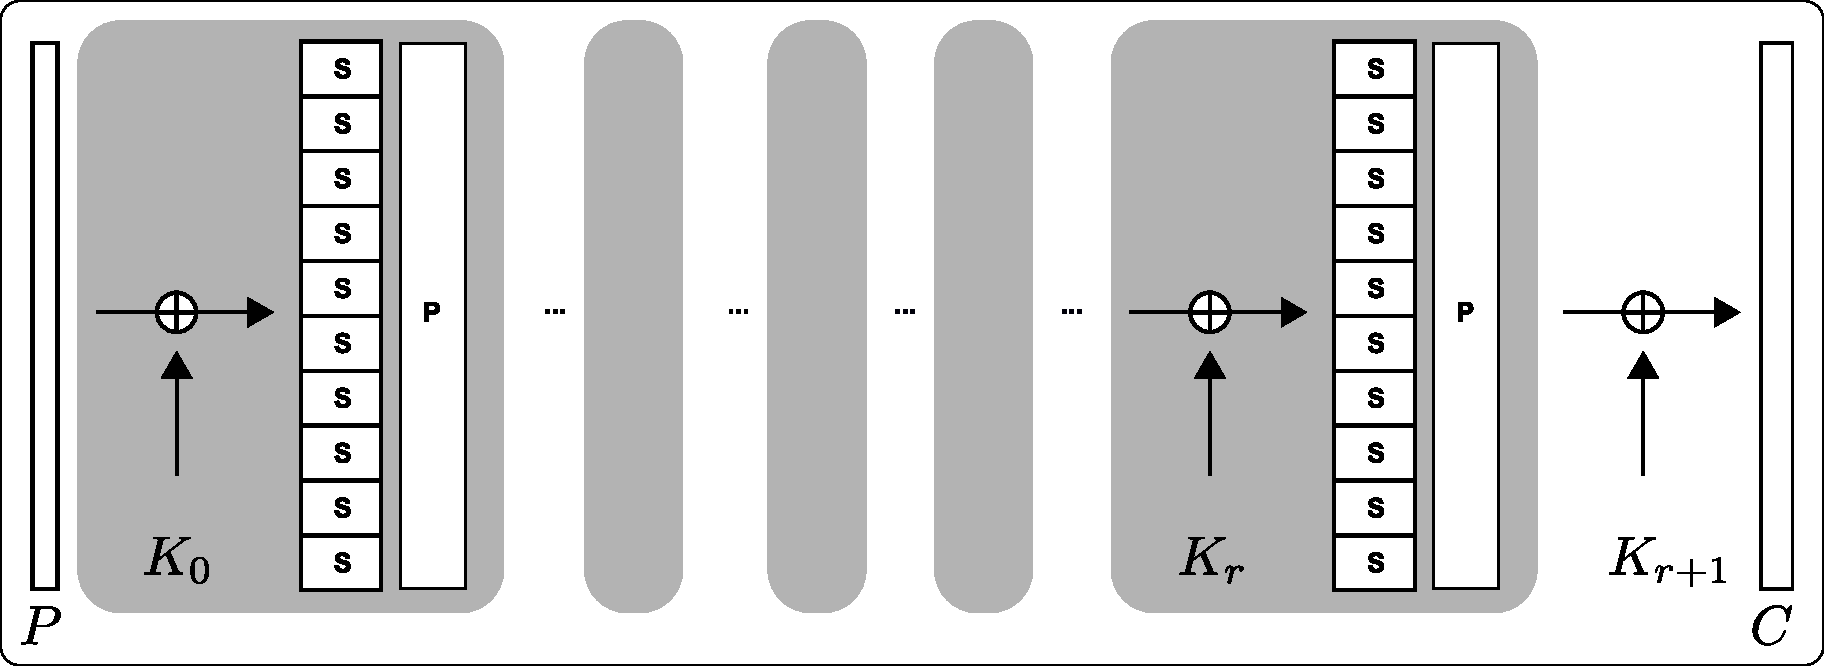
\includegraphics[width=1.0\textwidth]{./spn-scheme.pdf}
\end{center}
\end{frame}

\begin{frame}
\frametitle{Key Addition and the Permutation Layer}

\begin{itemize}
  \item \emph{Key addition} is easy, if $X_i$ is a bit before key addition and $Y_i$ is a bit after key addition, we write:
\[Y_i + X_i + K_i (=0).\]
  \item the \emph{Permutation layer} is just a permutation of wires given by the rule
\[s \cdot j + i \Rightarrow  B \cdot i + j \textnormal{ for } 0 \leq j < 16 \textnormal{ and } 0 \leq i < 4,\] hence we simply rename variables.
\end{itemize}

\end{frame}

\begin{frame}[allowframebreaks,fragile]
\frametitle{S-Box}
\begin{columns}

\column{0.5\textwidth}

The S-box is a non-linear operation. However, finding equations is still easy.

\vspace{1em}

As an example consider the 3-bit (since it fits on the slides) S-box 

$$[7,6,0,4,2,5,1,3].$$

\vspace{1em}

Construct the matrix on the right and perform Gaussian elimination on it.

\column{0.5\textwidth}
\begin{small}
\begin{align*}
\begin{array}{rrrrrrrrrr}
0\ & 1 & 2\  & 3 & 4\  & 5 & 6 & 7 & \ \ \ \ \ \ \ \ \ \ \\
\end{array}\\
\left(\begin{array}{rrrrrrrr|r}
1 & 1 & 1 & 1 & 1 & 1 & 1 & 1 & 1 \\
0 & 0 & 0 & 0 & 1 & 1 & 1 & 1 & x_{0} \\
0 & 0 & 1 & 1 & 0 & 0 & 1 & 1 & x_{1} \\
0 & 1 & 0 & 1 & 0 & 1 & 0 & 1 & x_{2} \\
1 & 1 & 0 & 1 & 0 & 1 & 0 & 0 & y_{0} \\
1 & 1 & 0 & 0 & 1 & 0 & 0 & 1 & y_{1} \\
1 & 0 & 0 & 0 & 0 & 1 & 1 & 1 & y_{2} \\
0 & 0 & 0 & 0 & 0 & 0 & 1 & 1 & x_{0} x_{1} \\
0 & 0 & 0 & 0 & 0 & 1 & 0 & 1 & x_{0} x_{2} \\
0 & 0 & 0 & 0 & 0 & 1 & 0 & 0 & x_{0} y_{0} \\
0 & 0 & 0 & 0 & 1 & 0 & 0 & 1 & x_{0} y_{1} \\
0 & 0 & 0 & 0 & 0 & 1 & 1 & 1 & x_{0} y_{2} \\
0 & 0 & 0 & 1 & 0 & 0 & 0 & 1 & x_{1} x_{2} \\
0 & 0 & 0 & 1 & 0 & 0 & 0 & 0 & x_{1} y_{0} \\
0 & 0 & 0 & 0 & 0 & 0 & 0 & 1 & x_{1} y_{1} \\
0 & 0 & 0 & 0 & 0 & 0 & 1 & 1 & x_{1} y_{2} \\
0 & 1 & 0 & 1 & 0 & 1 & 0 & 0 & x_{2} y_{0} \\
0 & 1 & 0 & 0 & 0 & 0 & 0 & 1 & x_{2} y_{1} \\
0 & 0 & 0 & 0 & 0 & 1 & 0 & 1 & x_{2} y_{2} \\
1 & 1 & 0 & 0 & 0 & 0 & 0 & 0 & y_{0} y_{1} \\
1 & 0 & 0 & 0 & 0 & 1 & 0 & 0 & y_{0} y_{2} \\
1 & 0 & 0 & 0 & 0 & 0 & 0 & 1 & y_{1} y_{2}
\end{array}\right)
\end{align*}
\end{small}
\end{columns}
\begin{small}
\begin{align*}
\left(\begin{array}{rrrrrrrr|r}
1 & 0 & 0 & 0 & 0 & 0 & 0 & 0 & x_{0} y_{0} + x_{1} + x_{2} + y_{0} + y_{1} + 1\\
0 & 1 & 0 & 0 & 0 & 0 & 0 & 0 & x_{0} y_{0} + x_{0} + x_{1} + y_{2} + 1 \\
0 & 0 & 1 & 0 & 0 & 0 & 0 & 0 & x_{0} y_{0} + x_{0} + y_{0} + 1 \\
0 & 0 & 0 & 1 & 0 & 0 & 0 & 0 & x_{0} y_{0} + x_{0} + x_{2} + y_{1} + y_{2} \\
0 & 0 & 0 & 0 & 1 & 0 & 0 & 0 & x_{0} y_{0} + x_{0} + x_{1} + x_{2} + y_{0} + y_{1} + y_{2} + 1 \\
0 & 0 & 0 & 0 & 0 & 1 & 0 & 0 & x_{0} y_{0} \\
0 & 0 & 0 & 0 & 0 & 0 & 1 & 0 & x_{0} y_{0} + x_{2} + y_{0} + y_{2} \\
0 & 0 & 0 & 0 & 0 & 0 & 0 & 1 & x_{0} y_{0} + x_{1} + y_{1} + 1 \\
0 & 0 & 0 & 0 & 0 & 0 & 0 & 0 & {\color{oxygenorange}x_{0} x_{2} + x_{1} + y_{1} + 1} \\
0 & 0 & 0 & 0 & 0 & 0 & 0 & 0 & {\color{oxygenorange}x_{0} x_{1} + x_{1} + x_{2} + y_{0} + y_{1} + y_{2} + 1} \\
0 & 0 & 0 & 0 & 0 & 0 & 0 & 0 & {\color{oxygenorange}x_{0} y_{1} + x_{0} + x_{2} + y_{0} + y_{2}} \\
0 & 0 & 0 & 0 & 0 & 0 & 0 & 0 & {\color{oxygenorange}x_{0} y_{0} + x_{0} y_{2} + x_{1} + x_{2} + y_{0} + y_{1} + y_{2} + 1} \\
0 & 0 & 0 & 0 & 0 & 0 & 0 & 0 & {\color{oxygenorange}x_{1} x_{2} + x_{0} + x_{1} + x_{2} + y_{2} + 1} \\
0 & 0 & 0 & 0 & 0 & 0 & 0 & 0 & {\color{oxygenorange}x_{0} y_{0} + x_{1} y_{0} + x_{0} + x_{2} + y_{1} + y_{2}} \\
0 & 0 & 0 & 0 & 0 & 0 & 0 & 0 & {\color{oxygenorange}x_{0} y_{0} + x_{1} y_{1} + x_{1} + y_{1} + 1} \\
0 & 0 & 0 & 0 & 0 & 0 & 0 & 0 & {\color{oxygenorange}x_{1} y_{2} + x_{1} + x_{2} + y_{0} + y_{1} + y_{2} + 1} \\
0 & 0 & 0 & 0 & 0 & 0 & 0 & 0 & {\color{oxygenorange}x_{0} y_{0} + x_{2} y_{0} + x_{1} + x_{2} + y_{1} + 1} \\
0 & 0 & 0 & 0 & 0 & 0 & 0 & 0 & {\color{oxygenorange}x_{2} y_{1} + x_{0} + y_{1} + y_{2}} \\
0 & 0 & 0 & 0 & 0 & 0 & 0 & 0 & {\color{oxygenorange}x_{2} y_{2} + x_{1} + y_{1} + 1} \\
0 & 0 & 0 & 0 & 0 & 0 & 0 & 0 & {\color{oxygenorange}y_{0} y_{1} + x_{0} + x_{2} + y_{0} + y_{1} + y_{2}} \\
0 & 0 & 0 & 0 & 0 & 0 & 0 & 0 & {\color{oxygenorange}y_{0} y_{2} + x_{1} + x_{2} + y_{0} + y_{1} + 1} \\
0 & 0 & 0 & 0 & 0 & 0 & 0 & 0 & {\color{oxygenorange}y_{1} y_{2} + x_{2} + y_{0}}
\end{array}\right)              
\end{align*}
\end{small}


\framebreak

If you cannot be bothered to do that yourself, use Sage:

\begin{lstlisting}
sage: S = mq.SBox(7,6,0,4,2,5,1,3) # 3-bit S-box
sage: S.polynomials()
[x0*x2 + x1 + y1 + 1, 
 x0*x1 + x1 + x2 + y0 + y1 + y2 + 1, 
 x0*y1 + x0 + x2 + y0 + y2, 
 x0*y0 + x0*y2 + x1 + x2 + y0 + y1 + y2 + 1, 
 x1*x2 + x0 + x1 + x2 + y2 + 1, 
 x0*y0 + x1*y0 + x0 + x2 + y1 + y2, 
 x0*y0 + x1*y1 + x1 + y1 + 1,
 x1*y2 + x1 + x2 + y0 + y1 + y2 + 1,
 x0*y0 + x2*y0 + x1 + x2 + y1 + 1,
 x2*y1 + x0 + y1 + y2,
 x2*y2 + x1 + y1 + 1,
 y0*y1 + x0 + x2 + y0 + y1 + y2,
 y0*y2 + x1 + x2 + y0 + y1 + 1,
 y1*y2 + x2 + y0]
\end{lstlisting}

If we post-process these polynomials (\lstinline{groebner=True}), we get 21 quadratic equations and one cubic equation for the S-Box which have a nice algebraic structure.

\end{frame}

\begin{frame}[fragile]
\frametitle{Putting it all together} 

\begin{itemize}
 \item We have equations for the $S$ layer, $P$ layer and the key addtion.
 \item The key schedule is similar and has one/two S-boxes. 
 \item For each round we introduce $2 \cdot 64$ new state variables for the $S$ layer.
 \item Adding key schedule and key variables we get $132 \cdot Nr +80$ variables
 \item On ther other hand, we get $(22 ⋅ 16 + 22 + 64)Nr + 64$ equations
\end{itemize}

\begin{lstlisting}
sage: s='https://bitbucket.org/malb/research-snippets/raw/tip/present.py'
sage: load(s)
sage: p = PRESENT(Nr=31)
sage: F,s = p.polynomial_system(); F
Polynomial System with 13642 Polynomials in 4172 Variables
\end{lstlisting}

\begin{block}{}
Solving this system means recovering the key \dots
\end{block}
\end{frame}


\subsection{Solvers}

\begin{frame}
\frametitle{Solver Families} 

\vfill

Three families of algorithms are popular in cryptography:

\vspace{1em}

\begin{enumerate}
 \item SAT solvers: MiniSat2, CryptoMiniSat \dots
 \item Gröbner basis methods: Buchberger's algorithm, F$_4$, F$_5$, \dots
 \item Mixed Integer (Linear) Solvers: SCIP, CPLEX, Gurobi, \dots
\end{enumerate}

\vspace{1em}

It is very useful to understand a bit how these solvers work.

\vspace{1em}

\begin{block}{not a valid analysis:}
``We put our equations into \textsc{Magma} and it ran out of memory.''
\end{block}

\vfill

\end{frame}


\begin{frame}[allowframebreaks,fragile]
\frametitle{Gröbner Bases}
\framesubtitle{for Cryptographers} 

\begin{itemize}
 \item $\field{F}_q$ is a finite field of order $q$.
 \item $P = \field{F}_q[x_1,\dots,x_{n}]$.
 \item $\mathcal{I}$ is an ideal $ \subset P$. That is, $f,g \in \mathcal{I} \rightarrow f + g \in \mathcal{I}$ and $f \in P, g \in \mathcal{I} \rightarrow f \cdot g \in \mathcal{I}.$
 \item $\ideal{f_1,\dots,f_{m}}$ is the ideal spanned by $f_1,\dots,f_{m}$.
\begin{lstlisting}
sage: P.<x,y,z> = PolynomialRing(GF(127),order='deglex')
sage: I = ideal(x*y + z, y^3 + 1, z^2 - x*5 - 1)
sage: (x*y + z) + (y^3 + 1) in I
True
sage: x*z*(z^2 - x*5 - 1) in I
True
\end{lstlisting}

A familiar example:
\begin{lstlisting}
sage: I = ideal([5]); I
Principal ideal (5) of Integer Ring
sage: 5 + 10 in I
True
sage: 3*5 in I
True
\end{lstlisting}



\framebreak 
 \item A term order decides how we compare monomials, e.g., is $xy$ or $y^3$ bigger\\(e.g.\ degree or variable first)?
\begin{lstlisting}
sage: P.<x,y,z> = PolynomialRing(GF(127),order='lex')
sage: x*y > y^3 # variable then degree
True
sage: P.<x,y,z> = PolynomialRing(GF(127),order='deglex')
sage: x*y > y^3 # degree then variable
False
\end{lstlisting}
 \item $\M{f}$ is the set of all monomials in $f$.
 \item $\LM{f}$ is the leading or largest monomial in $f$.
\begin{lstlisting}
sage: P.<x,y,z> = PolynomialRing(GF(127),order='deglex')
sage: f = x*y + x + 3
sage: f.lm()
x*y
sage: f.monomials()
[x*y, x, 1]
\end{lstlisting}
\end{itemize}

\framebreak

\begin{definition}[Gr\"obner Basis]
Let $\mathcal{I}$ be an ideal in $\field{F}[x_1,\dots,x_{n}]$ and fix a monomial ordering. A finite subset $$G = \{g_1 ,\dots , g_{m} \} \subset \mathcal{I}$$  is said to be a \emph{Gr\"obner basis} of $\mathcal{I}$ if for any $f \in \mathcal{I}$ there exists $g_i \in G$ such that $$\LM{g_i} \mid \LM{f}.$$
\end{definition}

\framebreak

Gröbner bases generalise greatest common divisors over $\field{F}[x]$ and\\row echelon forms over $\field{F}^n$.

\begin{lstlisting}
sage: P.<x,y,z> = PolynomialRing(GF(7), order='deglex')
sage: F = Sequence([ -x*y - x*z - 2*z^2 - 2*y,  
                      x*y + 2*y*z - 2*z^2 - x - 2*y,  
                      z^2 + 2*x + 3*y - 3*z - 3])
sage: map(lambda f: f.lm(), F.groebner_basis())
[y^3, y^2*z, x^2, x*y, x*z, z^2]

# GCD
sage: R.<x> = PolynomialRing(GF(7))
sage: f = x^2 + 6
sage: I = Ideal(map(P, [R.random_element() * f for _ in range(5)]))
sage: I.groebner_basis()
[x^2 - 1]

# Echelon Form
sage: F = Sequence([-3*y, -2*x - y - 3*z + 2, x + y + 2*z - 1])
sage: F.groebner_basis()
[x - 1, y, z]
sage: A,v = F.coefficient_matrix()
sage: A.echelonize()
sage: (A*v).T
[x - 1     y     z]
\end{lstlisting}


\framebreak

As a warm-up, consider a linear system of equations over $\field{F}_{127}[x,y,z]$.

\begin{columns}
\column{0.5\textwidth}
\begin{align*}
f &= 26y + 52z + 62 = 0\\
g &= 54y + 119z + 55 = 0\\
h &= 41x + 91z + 13 = 0
\end{align*}
\ After Gaussian elimination:
\begin{align*}
f' &= x + 29 = 0\\
g' &= y + 38 = 0\\
h' &= z + 75 = 0
\end{align*}
\column{0.5\textwidth}
\begin{align*}
\left(\begin{array}{rrrr}
0 & 26 & 52 & 62 \\
0 & 54 & 119 & 55 \\
41 & 0 & 91 & 13
\end{array}\right)
\end{align*}
\ \\
\begin{align*}
\left(\begin{array}{rrrr}
1 & 0 & 0 & 29 \\
0 & 1 & 0 & 38 \\
0 & 0 & 1 & 75
\end{array}\right)
\end{align*}
\end{columns}

\vspace{1em}

Thus, $x = -29$, $y = - 38$ and $z = - 75$ is a solution. We know this because Gaussian elimination produced small enough elements ($z + 75$) such that we can simply read of the solution.

\vspace{1em}

\framebreak

Now consider two polynomials in $\field{F}_{127}[x,y,z]$ with term ordering \textbf{deglex}.

\begin{columns}
\column{0.5\textwidth}
\begin{align*}
f &= x^2 + 2xy - 2y^2 + 14z^2 + 22z\\
g &= x^2 + xy + y^2 + z^2 + x + 2z
\end{align*}
\begin{align*}
f &= x^2 + 4 y^2  -12 z^2 + 2 x - 18 z \\
g'&= x y + -3 y^{2} + 13 z^{2} - x + 20 z
\end{align*}
\column{0.5\textwidth}
\begin{align*}
\left(\begin{array}{rrrrrr}
1 & 2 & -2 & 14 & 0 & 22 \\
1 & 1 &  1 &  1 & 1 &  2
\end{array}\right)
\end{align*}
\begin{align*}
\left(\begin{array}{rrrrrr}
1 & 0 &  4 & -12 &  2 & -18 \\
0 & 1 & -3 &  13 & -1 &  20
\end{array}\right)
\end{align*}
\end{columns}

\vspace{1em}

\begin{block}{}
Gaussian elimination still ``reduces'' the system.
\end{block}


\framebreak

This approach fails for
\begin{align*}
f &= {\color{oxygenorange}x^2} - 2{\color{oxygenorange}xy} - 2y^2 + 14z^2,\\
g &= {\color{oxygenorange}x} + y + 2z.
\end{align*}
since ${\color{oxygenorange}x}$ is not a monomial of $f$. 

\vspace{1em}

However, $x$ divides two monomials of $f$: ${\color{oxygenorange}x^2}$ and ${\color{oxygenorange}xy}$. 

\vspace{1em}

To account for those include multiples $m \cdot g$ of $g$ such that $$\LM{m \cdot g} = m \cdot \LM{g} \in \M{f}.$$

\framebreak

\begin{columns}
\column{0.4\textwidth}
\begin{align*}
f &= x^2 - 2xy - 2y^2 + \dots \\
x \cdot g &= {\color{oxygenorange}x^{2}} + x y \dots\\
y \cdot g &= {\color{oxygenorange}xy} + y^{2} + \dots\\
g &= x + y + 2z
\end{align*}
\begin{align*}
f' &= x^{2} + 4 y z + 14 z^{2},\\
h_1 &= {\color{oxygenorange}x y} + 2 x z + -4 y z - \dots,\\
h_2 &= {\color{oxygenorange}y^{2}} -2 x z + 6 y z + \dots,\\
g &= x + y + 2 z
\end{align*}
\column{0.6\textwidth}
\begin{align*}
\left(\begin{array}{rrrrrrrrr}
1 & -2 & -2 & 0 & 0 & 14 & 0 & \dots \\
1 & 1 & 0 & 2 & 0 & 0 & 0 & \dots \\
0 & 1 & 1 & 0 & 2 & 0 & 0 & \dots \\
0 & 0 & 0 & 0 & 0 & 0 & 1 & \dots
\end{array}\right)
\end{align*}
\begin{align*}
\left(\begin{array}{rrrrrrr}
1 & 0 & 0 & 0 & \dots & 0 & \dots \\
0 & 1 & 0 & 2 & \dots & 0 & \dots \\
0 & 0 & 1 & -2 &\dots & 0 & \dots \\
0 & 0 & 0 & 0  &\dots & 1 & \dots
\end{array}\right)
\end{align*}
\end{columns}

\vspace{1em}

Let's call the preprocessing we performed ``symbolic preprocessing'' \dots but that alone is still not enough to solve the system.


\framebreak

Finally, consider 
\begin{eqnarray*}
f &=& yx + 1,\\
g &=& zx + 2.
\end{eqnarray*}
Neither $\LM{f}$ nor $\LM{g}$ divides any monomial in the other polynomial. However, we have

\begin{eqnarray*}
zf - yg &=& z(yx + 1) - y(zx + 2),\\
        &=& {\color{oxygenorange}xyz} + z - {\color{oxygenorange}xyz} - 2y,\\
        &=& z - 2y.
\end{eqnarray*}

We constructed multiples of $f$ and $g$ such that when we subtract them their leading terms cancel out and something smaller is produced: we constructed an \emph{S-polynomial}.

\framebreak

\begin{definition}[S-Polynomial]
\label{def:spolynomials}
Let $f,g\ \in\ \field{F}[x_1,\dots,x_{n}]$ be non-zero polynomials.
\begin{itemize}
\item  Let $x^\gamma$ be the least common multiple of $\LM{f}$ and $\LM{g}$, written as $$x^\gamma\ =\LCM{\LM{f},\LM{g}}.$$  
\item The S-polynomial of $f$ and $g$ is defined as
$$
S(f,g)\ =\ \frac{x^\gamma}{\textsc{LT}(f)}\cdot f\ -\
\frac{x^\gamma}{\textsc{LT}(g)}\cdot g.
$$
\end{itemize}
\end{definition}

\framebreak

\begin{block}{}
It is \emph{sufficient} to consider \emph{only} S-polynomials since \emph{any} reduction of leading terms can be attributed to S-polynomials. 
\end{block}

\vspace{1em}

\begin{thebibliography}{fooobaaa}
\bibitem{Buc64}[Buc65] Bruno Buchberger
\newblock Ein {A}lgorithmus zum {A}uffinden der {B}asiselemente des {R}estklassenrings nach einem nulldimensionalen {P}olynomideal,
\newblock Phd Thesis at Universität Innsbruck, 1965.

\bibitem{Buc06}[Buc06] Bruno Buchberger
\newblock Bruno Buchberger's PhD thesis 1965: An algorithm for finding the basis elements of the residue class ring of a zero dimensional polynomial ideal
\newblock Journal of Symbolic Computation, 41:3-4, p.\ 475-511, 2006.

\end{thebibliography}


\framebreak

\begin{algorithm}[H]
\KwIn{$F = [f_1,\dots,f_{m}]$ -- list of polynomials}
\KwOut{a Gröbner basis for $\ideal{f_1,\dots,f_{m-1}}$}
\Begin{
 \While{True}{
   $\overline{F} \gets $ multiply all pairs $f_i,f_j \in F$ by $m_i,m_j$ such that $\LM{m_if_i} = \LM{m_jf_j}$\nllabel{select}\;
   $\overline{F} \gets $ perform ``symbolic preprocessing'' on $\overline{F} \cup F$\nllabel{symbolic}\;
   $\tilde F \gets$ peform Gaussian elimination on $\overline{F}$ \nllabel{elim}\;
   $F \gets F \cup \{f \in \tilde F \textnormal{ with } \forall g \in F \textnormal{ we have } \LM{g} \nmid \LM{f}\}$\;
   \If{$F$ didn't change in the last iteration}{
    \Return{$F$}\;
   }
 }
} 
\caption{simplified $F_4$}
\label{alg:f4o}
\end{algorithm}

\framebreak

\begin{algorithm}[H]
\Begin{
 \While{True}{
   $\overline{F} \gets $ multiply all pairs $f_i,f_j \in F$ by $m_i,m_j$ such that $\LM{m_if_i} = \LM{m_jf_j}$\;
   $\overline{F} \gets $ perform ``symbolic preprocessing'' on $\overline{F} \cup F$\;
   $\tilde F \gets$ peform Gaussian elimination on $\overline{F}$\;
   $F \gets F \cup \{f \in \tilde F \textnormal{ with } \forall g \in F \textnormal{ we have } \LM{g} \nmid \LM{f}\}$\;
   \If{$F$ didn't change in the last iteration}{
    \Return{$F$}\;
   }
 }
} 
\end{algorithm}

{\small
\begin{description}
 \item[Buchberger] select one pair in line~\ref{select} and use polynomial division instead of Gaussian elimination in line~\ref{elim}; implemented everywhere
 \item[F$_4$] use Buchberger's criteria in line~\ref{select} to avoid useless pairs (= zero rows in the matrix); implemented in \textsc{Magma}, \textsc{PolyBoRi}, FGB
 \item[F$_5$] use criteria in lines~\ref{select} and \ref{symbolic} such that all matrices have full rank under some assumption; implementation worked on in \textsc{Singular}
\end{description}}

\framebreak

\begin{algorithm}[H]
\Begin{
 \While{True}{
   $\overline{F} \gets $ multiply all pairs $f_i,f_j \in F$ by $m_i,m_j$ such that $\LM{m_if_i} = \LM{m_jf_j}$\;
   $\overline{F} \gets $ perform ``symbolic preprocessing'' on $\overline{F} \cup F$\;
   $\tilde F \gets$ peform Gaussian elimination on $\overline{F}$\;
   $F \gets F \cup \{f \in \tilde F \textnormal{ with } \forall g \in F \textnormal{ we have } \LM{g} \nmid \LM{f}\}$\;
   \If{$F$ didn't change in the last iteration}{
    \Return{$F$}\;
   }
 }
} 
\end{algorithm}

{\small
\begin{description}
 \item[(Mutant)XL] multiply by everything up to some degree in line~\ref{select} and skip line~\ref{symbolic} (worse than Algorithm~\ref{alg:f4o} because of redundancies)
 \item[XSL] make some (very bad!) choice in line~\ref{select} and line~\ref{symbolic} (worse than Algorithm~\ref{alg:f4o} because of bad choices)
 \item[ElimLin] always stay at degree 2 $\rightarrow$ line~\ref{symbolic} + line~\ref{elim} (less powerful than Algorithm~\ref{alg:f4o})
\end{description}}


\end{frame}

\begin{frame}[fragile,allowframebreaks]
\frametitle{Gröbner Bases in Sage}

Let's play a bit with Gröbner bases in Sage:

\begin{lstlisting}
sage: K = GF(32003)
sage: T = TermOrder("deglex",2) + TermOrder("deglex",2)
sage: P.<w,x,y,z> = PolynomialRing(K,order=T)
sage: I = sage.rings.ideal.Katsura(P)
sage: [g.lm() for g in I.groebner_basis()] # Singular
[w, x, y*z^3, z^4, y^3, y^2*z]
sage: I.dimension() # finite number of solutions
0
sage: V = I.variety(); V # solutions
[{y: 0, z: 0, w: 1, x: 0}, {y: 0, z: 10668, w: 10668, x: 0}]
sage: J = I.change_ring(P.change_ring(QQ))  # over the rationals
sage: J.variety()
[{y: 0, z: -32002/3, w: -32002/3, x: 0}, {y: 0, z: 0, w: -32002, x: 0}]
sage: len(J.variety(CC)) # over the complex numbers
8
\end{lstlisting}

\framebreak

We estimate the complexity before solving:

\begin{lstlisting}
sage: n = 10; P = PolynomialRing(GF(32003), n, 'x')
sage: F = [P.random_element() for _ in range(P.ngens()+2)]
sage: s = random_vector(GF(32003),n)
sage: I = Ideal(f-f(*s) for f in F)
sage: D = I.degree_of_semi_regularity()
sage: D, log(binomial(n + D, n)^3, 2).n() # prediction: degree six
6, 34.65...
sage: I.groebner_basis('magma',prot='sage')
...
Leading term degree:  4. Critical pairs: 178.
Leading term degree:  5. Critical pairs: 515.
Leading term degree:  5. Critical pairs: 1155.
Leading term degree:  3. Critical pairs: 2845.
Leading term degree:  2. Critical pairs: 2850.
Leading term degree:  3. Critical pairs: 2795.
Leading term degree:  4. Critical pairs: 2605.
Leading term degree:  5. Critical pairs: 1609.
Leading term degree:  6. Critical pairs: 864 (all pairs ...
Leading term degree:  7. Critical pairs: 4 (all pairs ...
Leading term degree:  8. Critical pairs: 1 (all pairs ...

Highest degree reached during computation:  5.
[x0 + 7334, x1 - 12304, x2 - 7977, x3 - 8365, x4 - 7982, x5 + 676, ...]
\end{lstlisting}

\framebreak

Sage has a very good implementation of Gröbner basis computations over $\F_2[x_1,\dots,x_{n}]/\langle x_1^2 + x_1, \dots, x_{n}^2 + x_{n}\rangle$ thanks to {\tt PolyBoRi}.

\begin{lstlisting}
sage: B = BooleanPolynomialRing(50,'x',order='deglex')
sage: s = random_vector(GF(2),50)
sage: F = [B.random_element() for _ in range(500)]
sage: I = Ideal(f-f(*s) for f in F)
sage: G = I.groebner_basis(); G # PolyBoRi
Polynomial Sequence with 50 Polynomials in 50 Variables
sage: sorted(G)[0], s[0]
(x0 + 1, 1)
sage: I.variety()
[{x40: 0, x42: 1, x44: 0, ..., x23: 0, x25: 1}]
\end{lstlisting}

\end{frame}



\begin{frame}[fragile,allowframebreaks]
\frametitle{SAT Solvers} 

\begin{itemize}
 \item The SAT problem is a decision problem, whose instance is a Boolean expression written using only AND, OR, NOT, variables, and parentheses.
 \item The question is: given the expression, is there some assignment of TRUE and FALSE values to the variables that will make the entire expression true? 
 \item A \emph{literal} is either a variable or the negation of a variable
 \item A \emph{clause} is a disjunction of literals ($\vee =$ OR).
 \item A formula is in \emph{Conjunctive Normal Form} (CNF) if is a conjunction ($\wedge =$  AND) of clauses.
\end{itemize}

\begin{columns}
\column{0.2\textwidth}
\begin{eqnarray*}
&& x_1 \vee \neg x_2 \vee x_3\\
&& \neg x_1 \vee \neg x_3\\
\end{eqnarray*}
\column{0.7\textwidth}
\begin{lstlisting}
sage: from sage.sat.solvers import CryptoMiniSat 
sage: cms = CryptoMiniSat()
sage: cms.add_clause( (1, -2, 3) )
sage: cms.add_clause( (-1, -3) )
\end{lstlisting}
\end{columns}

\framebreak

We can solve (Boolean) polynomial systems using SAT solvers using ANF to CNF conversion:

\begin{lstlisting}
sage: import sage.sat.converters as satconv
sage: from satconv.polybori import CNFEncoder
sage: from sage.sat.solvers import CryptoMiniSat 
sage: B.<a,b> = BooleanPolynomialRing()
sage: cms = CryptoMiniSat()
sage: ce = CNFEncoder(cms, B)
sage: ce([a*b + b +1])
[None, a, b]
sage: cms.clauses()
[((2,), False, None), ((-1,), False, None)]
\end{lstlisting}

\begin{small}
\begin{thebibliography}{Bard2007a}
\bibitem{Bard2007a}
Gregory~V. Bard, Nicolas~T. Courtois, and Chris Jefferson.
\newblock {E}fficient {M}ethods for {C}onversion and {S}olution of {S}parse
  {S}ystems of {L}ow-{D}egree {M}ultivariate {P}olynomials over {GF(2)} via
  {SAT}-{S}olvers.
\newblock Cryptology ePrint Archive, Report 2007/024, 2007.
 \end{thebibliography}
\end{small}

\framebreak
\begin{columns}

\column{0.4\textwidth}
\begin{algorithm}[H]
\Begin{
 \While{True}{
   simplify clauses\;
   \If{contradiction}{backtrack\;}
   \If{solution}{\Return{}\;}
   {guess something\;}
 }
} 
\end{algorithm}
\column{0.6\textwidth}
 
\begin{itemize}
 \item SAT solvers decide satisfiability, hence they will terminate once \emph{one} solution is found.
 \item \dots in contrast to Gröbner basis methods.
 \item SAT solvers are randomised: one success does not constitute an average running time.
 \item Run hundreds/thousands of experiments with lots of re-randomisation.
 \item The conversion from ANF to CNF can make a huge difference, Sage supports two strategies at the moment.
 \item Different solvers behave differently.
\end{itemize}
\end{columns}

\begin{lstlisting}
sage: from sage.sat.boolean_polynomials import solve as solve_sat
sage: sr = mq.SR(1,2,2,4,gf2=True,polybori=True)
sage: set_random_seed(1337^3)
sage: F,s = sr.polynomial_system()
sage: len(solve_sat(F))            
1
sage: len(solve_sat(F, n=infinity)) 
3
\end{lstlisting}
\end{frame}


\begin{frame}[fragile,allowframebreaks]
\frametitle{SAT Solvers in Sage}
Sage has an interface for SAT solving via \textbf{CryptoMiniSat} which supports XOR clauses\\

\begin{lstlisting}
sage: from sage.sat.solvers import CryptoMiniSat 
sage: cms = CryptoMiniSat(verbosity=3)
sage: cms.add_clause((1,2,-3)) # x1 OR x2 OR -x3
sage: cms.add_clause((1,-2,3)) # x1 OR -x2 OR x3 
sage: cms.add_xor_clause((1,2,3), 0) # (x1 XOR x2 XOR x3 = 1)
sage: cms.add_xor_clause((1,3), 1) # (x1 XOR x3 = 0)
sage: cms()
...
(None, True, True, True)
\end{lstlisting}

or via any solver supporting the \textbf{DIMACS} format\\
\begin{lstlisting}
sage: from sage.sat.boolean_polynomials import solve as solve_sat
sage: F,s = mq.SR(1,1,1,4,gf2=True,polybori=True).polynomial_system()
sage: solve_sat(F, solver=sage.sat.solvers.RSat)
[{k003: 0,  k002: 0,  k001: 1,  k000: 1,  ..., 
  k103: 0,  k102: 1,  k101: 0,  k100: 0}]
\end{lstlisting}

\framebreak

Sage can take care of the ANF to CNF conversion details:

\begin{lstlisting}
sage: load('https://bitbucket.org/malb/research-snippets/raw/tip/present.py')
sage: from sage.sat.boolean_polynomials import solve as solve_sat
sage: F,s = PRESENT(Nr=2).polynomial_system()                    
sage: sprime = solve_sat(F,s_verbosity=3)
\end{lstlisting}

\dots and also learn new equations using a SAT solver with early abort:

\begin{lstlisting}
sage: set_random_seed(2300)
sage: sr = mq.SR(1,4,4,4,gf2=True,polybori=True)
sage: F,s = sr.polynomial_system()
sage: from sage.sat.boolean_polynomials import learn as learn_sat
sage: H = learn_sat(F, s_maxrestarts=20, interreduction=True)
sage: H[-1]
k001503*s021*x011502 + s021*x011502 + k001503*x011502 + x011502
\end{lstlisting}
\end{frame}


\begin{frame}[fragile,allowframebreaks]
\frametitle{Mixed Integer Programming} 

\begin{itemize}
 \item MIP minimises (or maximises) a linear function $c^T x$ subject to linear equality and inequality constraints given by linear inequalities $$Ax ≤ b.$$
 \item We restrict some variables to integer values while others may take any real values.
 \item The main advantage of MIP solvers compared to other branch-and-cut solvers (SAT solvers etc.) is that they can relax the problem to an (easy) floating point problem.
 \item This allows to obtain lower and upper bounds for $c^T x$ which can be used to cut search branches.
 \item The non-linear generalisation is called Constraint Integer Programming (CIP).
 \item Solvers: {\tt CPLEX} \& {\tt Gurobi} (accademic licenses available), {\tt SCIP} ($\approx$ open-source)
\end{itemize}


\framebreak
 
We can convert a polynomial $f \in \field{F}_2[x_1,\dots,x_{n}]$ to MIP and then use an off-the-shelf MIP solver (in this example SCIP).

\begin{lstlisting}
sage: from sage.libs.scip.scip import SCIP # trac 10879
sage: B.<a,b,c> = BooleanPolynomialRing()
sage: f = a*c + a + b + c + 1
sage: s = SCIP(maximization=False,name="icebreak")
sage: boolean_polynomials(s, Sequence([f]))
down: {b: 1, c: 0, a: 2}
  up: {0: c, 1: b, 2: a}
sage: _ = s.solve()
sage: s.get_all_solutions()
[({0: 0.0, 1: 1.0, 2: 0.0, 3: 0.0}, 1.0)]
\end{lstlisting}

\begin{small}
\begin{thebibliography}{biviummip}
\bibitem{biviummip}
Julia Borghoff, Lars~R. Knudsen, and Mathias Stolpe.
\newblock {B}ivium as a {M}ixed-{I}nteger {L}inear programming problem.
\newblock In Matthew~G. Parker, editor, {\em Cryptography and Coding -- 12th
  IMA International Conference}, volume 5921 of {\em Lecture Notes in Computer
  Science}, pages 133--152, Berlin, Heidelberg, New York, 2009. Springer
  Verlag.
\end{thebibliography}
\end{small}
\end{frame}

\begin{frame}[fragile]
\frametitle{Mixed Integer Programming in Sage}

Sage also has a highlevel interface to Mixed Integer Linear solving

\begin{lstlisting}
sage: g = graphs.PetersenGraph()
sage: p = MixedIntegerLinearProgram(maximization=True)
sage: b = p.new_variable()
sage: p.set_objective(sum([b[v] for v in g]))
sage: for (u,v) in g.edges(labels=None):
...       p.add_constraint(b[u] + b[v], max=1)
sage: p.set_binary(b)
sage: p.solve(objective_only=True)
4.0
\end{lstlisting}


which supports many backends: {\tt GLPK}, {\tt Coin}, {\tt Gurobi}, {\tt CPLEX}.

\end{frame}


\subsection{\dots for the Lazy Cryptographer}

\begin{frame}{Here's another picture of a kitten}
\begin{center}
 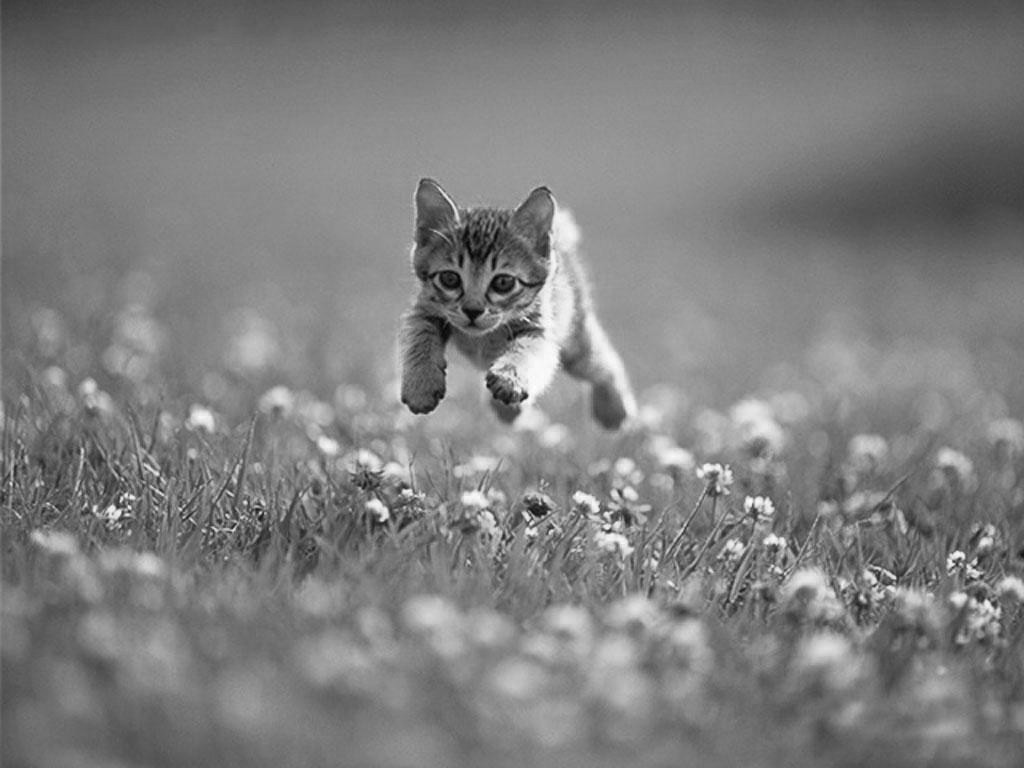
\includegraphics[width=0.9\textwidth]{./kitten-02.jpg}
 % kitten-02.jpg: 1024x768 pixel, 96dpi, 27.09x20.32 cm, bb=0 0 768 576
\end{center} 
\end{frame}


\begin{frame}[allowframebreaks,fragile]
\frametitle{Implications}
\framesubtitle{\dots or ``I cannot be bothered to work this out by hand''}
 
\begin{itemize}
\item Consider an arbitrary function \(f: \field{F}_2^n \to \field{F}_2^m\) and its boolean polynomial representation \(f_1, \dots, f_{m}\)
\item Let \(x_{1}, \dots x_{n}\) be the input variables and \(y_{1}, \dots, y_{m}\) the output variables
\item Consider the ideal \(\mathcal{I}= \langle f_1, \dots, f_{m}\rangle\):
\begin{itemize}
\item Every member \(g\) of this ideal is a combination of \( f_1, \dots, f_{m}\).
\item If \( f_{1}, \dots, f_{m}\) vanish, so does \(g\).
\end{itemize}
\end{itemize}           
\begin{block}{\( f_1, \dots, f_{m}\) implies \(g\)}
\begin{center}
``If \(f_1, \dots, f_{m}\) hold, so does \(g\)''.
\end{center}
\end{block}

\framebreak

\textbf{Example:} The \PRESENT S-box: [c, 5, 6, b, 9, 0, a, d, 3, e, f, 8, 4, 7, 1, 2]:

\begin{eqnarray*}
y_{0} &=& x_{0} x_{1} x_{3} + x_{0} x_{2} x_{3} + x_{0} + x_{1} x_{2} x_{3} + x_{1} x_{2} + x_{2} + x_{3} + 1,\\
y_{1} &=& x_{0} x_{1} x_{3} + x_{0} x_{2} x_{3} + x_{0} x_{2} + x_{0} x_{3} + x_{0} + x_{1} + x_{2} x_{3} + 1,\\
y_{2} &=& x_{0} x_{1} x_{3} + x_{0} x_{1} + x_{0} x_{2} x_{3} + x_{0} x_{2} + x_{0} + x_{1} x_{2} x_{3} + x_{2},\\
y_{3} &=& x_{0} + x_{1} x_{2} + x_{1} + x_{3}.
\end{eqnarray*}

\begin{lstlisting}
sage: S = mq.SBox(12,5,6,11,9,0,10,13,3,14,15,8,4,7,1,2)
sage: B.<y0,y1,y2,y3,x0,x1,x2,x3> = BooleanPolynomialRing(order='lex')
sage: X = (x0,x1,x2,x3); Y = (y0,y1,y2,y3)
sage: S.polynomials(X=X, Y=Y, degree=3, groebner=True)
[y0 + x0*x1*x3 + x0*x2*x3 + x0 + x1*x2*x3 + x1*x2 + x2 + x3 + 1,
 y1 + x0*x1*x3 + x0*x2*x3 + x0*x2 + x0*x3 + x0 + x1 + x2*x3 + 1,
 y2 + x0*x1*x3 + x0*x1 + x0*x2*x3 + x0*x2 + x0 + x1*x2*x3 + x2,
 y3 + x0 + x1*x2 + x1 + x3]
\end{lstlisting}

\framebreak

\begin{itemize}
\item Let \(c\) be a condition on the input variables (in polynomial form).
\vspace{1em} \\
\textbf{Example:} \hspace{3em} $x_0 = 1$\hspace{3em} \lstinline{sage: c = x0 + 1}

\framebreak

\item Calculate a Gr\"obner basis for \(\langle c, f_1, \dots, f_{m}\rangle\) in an elimination ordering which eliminates input variables first.

\begin{lstlisting}
sage: S = mq.SBox(12,5,6,11,9,0,10,13,3,14,15,8,4,7,1,2)
sage: BPRing = BooleanPolynomialRing 
sage: T = TermOrder('lex')
sage: B.<x0,x1,x2,x3,y0,y1,y2,y3> = BPRing(order=T) # x > y
sage: X = (x0,x1,x2,x3); Y = (y0,y1,y2,y3)
sage: F = Sequence( S.polynomials(X=X, Y=Y, degree=3) )
sage: c = x0 + 1
sage: F += [c]
sage: G = F.groebner_basis()
\end{lstlisting}

\framebreak

\item The smallest elements of this Gr\"obner basis will be polynomials with a minimum number of input variables (if possible, none). Call them \(g_0, \dots, g_{r-1}\).

\item These polynomials are \textbf{implied} by the polynomials \(f_1, \dots, f_{m}\) and the condition \(c\).
\end{itemize}           

\begin{block}{}
\begin{center}
``If \(f_1, \dots, f_{m}\) and the condition \(c\) hold, so do \(g_1, \dots, g_{r}\)''
\end{center}
\end{block}

\begin{lstlisting}
sage: G[-1]
y1*y2*y3 + y1*y3
\end{lstlisting}


\framebreak

\begin{itemize}
\item Moreover, \textbf{all} on the output bits that are implied by \(f\) under condition \(c\) are \textbf{combinations} of \(g_1, \dots, g_{r}\)
\item If we pick the term ordering right, $g_1,\dots,g_{r}$ have minimal degree.
\end{itemize}           
\begin{block}{}
For a given function \(f\) under a precondition \(c\) we can calculate \textbf{all}  conditions on the output bits that \textbf{must} hold.
\end{block}

\begin{lstlisting}
sage: S = mq.SBox(12,5,6,11,9,0,10,13,3,14,15,8,4,7,1,2)
sage: BPRing = BooleanPolynomialRing 
sage: T = TermOrder('deglex',4) + TermOrder('deglex',4) # order!
sage: B.<x0,x1,x2,x3,y0,y1,y2,y3> = BPRing(order=T) # x > y
sage: X = (x0,x1,x2,x3); Y = (y0,y1,y2,y3)
sage: F = Sequence( S.polynomials(X=X, Y=Y, degree=3) )
sage: c = x0 + 1
sage: F += [c]
sage: G = F.groebner_basis()
sage: G[4:]
[y1*y2*y3 + y1*y3,
 y0*y1 + y1*y2 + y2*y3 + y0 + y1 + y2 + y3 + 1,
 y0*y2 + y1*y2 + y2*y3 + y0 + y1 + y2 + y3 + 1,
 y0*y3 + y1*y3 + y2*y3 + y0 + y1 + y2 + y3 + 1]
\end{lstlisting}

\framebreak

\textbf{Applications:}      
\begin{description}
\item[Differential:] algebraic description of all possible output differences under some input difference.
\item[Cond.\ Diff.:]conditional relations on the plaintext and the key bits.
\item[Integral:] algebraic descriptions on the output bits after $r$ rounds.
\end{description}

\begin{small}
\begin{thebibliography}{inscrypt2010}
\bibitem{acdfp:inscrypt2010}
Martin Albrecht, Carlos Cid, Thomas Dullien, Jean-Charles Faugère, and Ludovic
  Perret.
\newblock Algebraic precomputations in Differential and Integral Cryptanalysis.
\newblock In {\em INSCRYPT 2010 -- {I}nformation {S}ecurity and {C}ryptology
  6th International Conference}, {\em Lecture Notes in Computer Science}, 18
  pages, October 2010.
\end{thebibliography}
 \end{small}

\end{frame}

\begin{frame}[allowframebreaks]
\frametitle{Algebraic Techniques and Integral Cryptanalysis} 

In integral or \emph{higher-order differential cryptanalysis} the attacker encrypts plaintexts with some structure such that the output (after some rounds) also has some (algebraic) structure. 

\framebreak

\begin{itemize}
 \item In \cite{bit-pattern-ia} \emph{bit-pattern based integral attacks} against up to 7 rounds of \PRESENT are proposed, based on a 3.5 round distinguisher.
 \item The attacker prepares 16 chosen plaintexts which agree in all bit values except the bits at the positions 51, 55, 59, 63. 
 \item These four bits take all possible values $(0,0,0,0),(0,0,0,1),\dots,(1,1,1,1)$. 
 \item Then he input bits to the 4th round are then balanced, i.e., the sum of all bits at the same bit position across all 16 encryptions is zero. 
 \item If $X_{i,j,k}$ denotes the $k$-th input bit of the $j$-th round of the $i$-th encryption, we have that $$0 = \sum_{i=0}^{15} X_{i,4,k} \textnormal{ for } 0 \leq k < 64.$$ 
\end{itemize}

\begin{thebibliography}{fooooo}
\bibitem[ZRHD08]{bit-pattern-ia}
Muhammad~Reza Z'Aba, Håvard Raddum, Matt Henricksen, and Ed~Dawson.
\newblock Bit-pattern based integral attacks.
\newblock In Kaisa Nyberg, editor, {\em {Fast Software Encryption} 2008},
  number 5086 in Lecture Notes In Computer Science, pages 363--381, Berlin,
  Heidelberg, New York, 2008. Springer Verlag.
\end{thebibliography}

\framebreak

I presume the result in \cite{bit-pattern-ia} was found by carefully tracing relations between bits through the cipher, I am too lazy for that.

\begin{itemize}
 \item Setup an equation system for the 16 plaintexts as in \cite{bit-pattern-ia},
 \item run a Gröbner basis computation up to degree $2$ under a term ordering where variables from small rounds are eliminated first.
 \item This produces 500 linear polynomials in $X_{i,4,k}$ and 26 linear polynomials in $X_{i,5,k}$
\end{itemize}

\begin{thebibliography}{fooooo}
\bibitem[Alb10]{phd}
Martin R.~Albrecht
\newblock Algorithmic Algebraic Techniques and their Application to Block Cipher Cryptanalysis
\newblock Phd Thesis at University of London, 2010
\end{thebibliography}

\framebreak

\begin{table}[htbp]
\begin{center}
\begin{tabular}{|r|r|r|r|}
\hline
Cipher & Method & \#P & Wall time\\
\hline
\PRESENT-80-5 &  HODC & $5\cdot 2^4$ & $\approx 2^{25.7}$ CPU cycles\\
\PRESENT-80-5 & AHODC & $2^4$ & $\approx 2^{23.3}$  CPU cycles\\
\PRESENT-80-6 &  HODC & $2^{22.4}$ & $\approx 2^{41.7}$  CPU cycles\\
\PRESENT-80-6 & AHODC & $2^{20}$ & $\approx 2^{39.3}$  CPU cycles\\
\PRESENT-80-7 &  HODC & $2^{24.4}$ & $\approx 2^{100.1}$  CPU cycles\\
\PRESENT-80-7 & AHODC & $2^{21.9}$ & $\approx 2^{97.8}$  CPU cycles\\
\hline
KTANTAN32-65 & AHODC & $2^5$& 59004.10~s\\
\hline
\end{tabular}
\end{center}
\end{table}
\end{frame}

\begin{frame}[allowframebreaks]
\frametitle{Designing Linear Layers}
\framesubtitle{\dots or ``I cannot be bothered to design an algorithm for that''}
\begin{itemize}
 \item Assume we have a (sparse) $n \times n$ matrix over $\F_2$ with a good differential branch number.
 \item We can use this matrix to construct an $2n \times 2n$ matrix over $\F_2$ with the same number of ones per row/column and branch number.
\end{itemize}

\begin{eqnarray*}
\left(\begin{array}{ccc}
a_{1,1} & \dots & a_{1,n}\\
\vdots  & \ddots &  \vdots\\
a_{n,1} & \dots & a_{n,n}\\
\end{array}\right)
\left(\begin{array}{ccc}
b_{1,1} & \dots & b_{1,n}\\
\vdots  & \ddots &  \vdots\\
b_{n,1} & \dots & b_{n,n}\\
\end{array}\right) \Rightarrow
\left(\begin{array}{cc|c|cc}
A_{1,1} & 0 & \dots & A_{1,n} & 0\\
0 & b_{1,1} & \dots & 0 & b_{1,n}\\
\hline
\vdots  & & \ddots & & \vdots\\
\hline
A_{n,1} & 0 & \dots & A_{n,n} & 0\\
0 & b_{n,1} & \dots & 0 & b_{n,n}\\
\end{array}\right)
\end{eqnarray*}

\begin{itemize}
 \item We want to avoid that both $a_{i,j} = b_{i,j = 0}$ to maximise diffusion.
\end{itemize}

\begin{block}{Task}
Find $B = P \cdot A \cdot Q$ such that diffusion is maximised where $P,Q$ are permutations.
\end{block}

\framebreak

We would go about this problem something like this:
\begin{enumerate}
 \item Try a bunch of random permutations and hope to get lucky (incomplete)
 \item Try some heuristic, such as local optimisation (incomplete)
 \item Run an exhaustive search over all permutation matrices, prunning search trees based on fill-in (complete, but takes a while to implement)
\end{enumerate}

\vspace{1em}

\dots or we can recognise this as a Constraint Integer Programming problem

\framebreak

We consider the matrices
\begin{eqnarray*}
P =  \left(\begin{array}{ccc}
                p_{1,1} & \dots & p_{1,n}\\
                \vdots & \ddots & \vdots\\
                p_{n,1} & \dots & p_{n,n}\\
                \end{array}\right),
Q =  \left(\begin{array}{ccc}
                q_{1,1} &  \dots & q_{1,n}\\
                \vdots  & \ddots & \vdots\\
                q_{n,1} & \dots & q_{n,n}\\
                \end{array}\right).
\end{eqnarray*}
where $p_{i,j}, q_{i,j}$ are boolean variables and denote
\begin{eqnarray*}
\left(\begin{array}{ccc}
                b_{1,1} & \dots  & b_{1,n}\\
                \vdots  & \ddots & \vdots\\
                b_{n,1} & \dots  & b_{n,n}\\
                \end{array}\right) = P \cdot A \cdot Q,
\end{eqnarray*}
We add 
\begin{enumerate}
 \item quadratic constraints expressing $b_{i,j}$ in terms of $P\cdot A \cdot Q$.
 \item linear constraints that all rows/columns of $P$ and $Q$ have exactly one $1$ per row/column.
 \item OR constraints $v_{i,j} = a_{i,j} \vee  b_{i,j}$.
\end{enumerate}
We then maximize $\sum v_{i,j}$ using an off-the-shelf CIP solver such as SCIP.

\framebreak

\begin{itemize}
 \item Including documentation, error checking, comments and generalised for arbitrarily many permutations of $A$ this takes about 100 lines of code to implement in Sage.
 \item It will run (much) slower than a dedicated algorithm or implementation.
\end{itemize}

\vspace{2em}

\begin{block}{Trade Off}
At what ratio do you ``trade'' CPU cycles and your time?
\end{block}
\end{frame}

\begin{frame}[allowframebreaks]
\frametitle{Algebraic Techniques and Side-Channel Cryptanalysis}
\framesubtitle{\dots or full ciphers are too hard}

\begin{itemize}
 \item Solving full ciphers seems way beyond what algebraic attacks can deliver.
 \item Side-channel attacks provide information about the internal state of an encryption operation to the attacker.
 \item This information can then be used to recover key information.
\end{itemize}

\framebreak

This means,
\begin{itemize}
 \item tracking information from the leak back to the key,
 \item where often only a limited number of readings are available, 
\end{itemize}
\dots so we might want to throw algebraic solvers at the problem.

\begin{block}{}
It is always possible to find a dedicated attack that is at least as good as the generic ``algebraic side-channel'' attack and plausibly one can often find dedicated attacks which are strictly better. Yet, the question is how hard it is to find these attacks.
\end{block}

\framebreak

\textbf{Example:} Power readings reveal information about S-box bits, combine these with cipher description and solve using a SAT solver.
\vspace{1em}
\begin{thebibliography}{}
\bibitem{alg-side-channel:eprint}
Mathieu Renauld and Francois-Xavier Standaert.
\newblock Algebraic Side-Channel Attacks.
\newblock In {\em INSCRYPT 2009 -- {I}nformation {S}ecurity and {C}ryptology 5th International Conference}, volume 6151 of {\em Lecture Notes in Computer Science}, pages 393-410, Berlin, Heidelberg, New York, 2009. Springer Verlag.
\end{thebibliography}
\framebreak

\textbf{Example:} Cold boot attacks recover noisy versions of the key schedule output, recover noise-free version via polynomial system solving with noise via Mixed Integer Programming.
\vspace{1em}
\begin{thebibliography}{}
\bibitem{coldboot}
Martin Albrecht and Carlos Cid.
\newblock Cold Boot Key Recovery by Solving Polynomial Systems with Noise 
\newblock In {\em ACNS 2011 -- 9th International Conference on Applied Cryptography and Network Security}, in {\em Lecture Notes in Computer Science}, Berlin, Heidelberg, New York, 2011. Springer Verlag.
\end{thebibliography}

\framebreak

\textbf{Example:} Fault attacks introduce a fault in the encryption and exploit the result wrong result, the key recovery can be accomplished using a SAT solver.
\vspace{1em}
\begin{thebibliography}{}
\bibitem{faultattack}
Philipp Jovanovic and Martin Kreuzer and Ilia Polian
\newblock An Algebraic Fault Attack on the LED Block Cipher
\newblock Cryptology ePrint Archive, Report 2012/400
\end{thebibliography}


\end{frame}

\begin{frame}{Questions?}

\begin{center}
 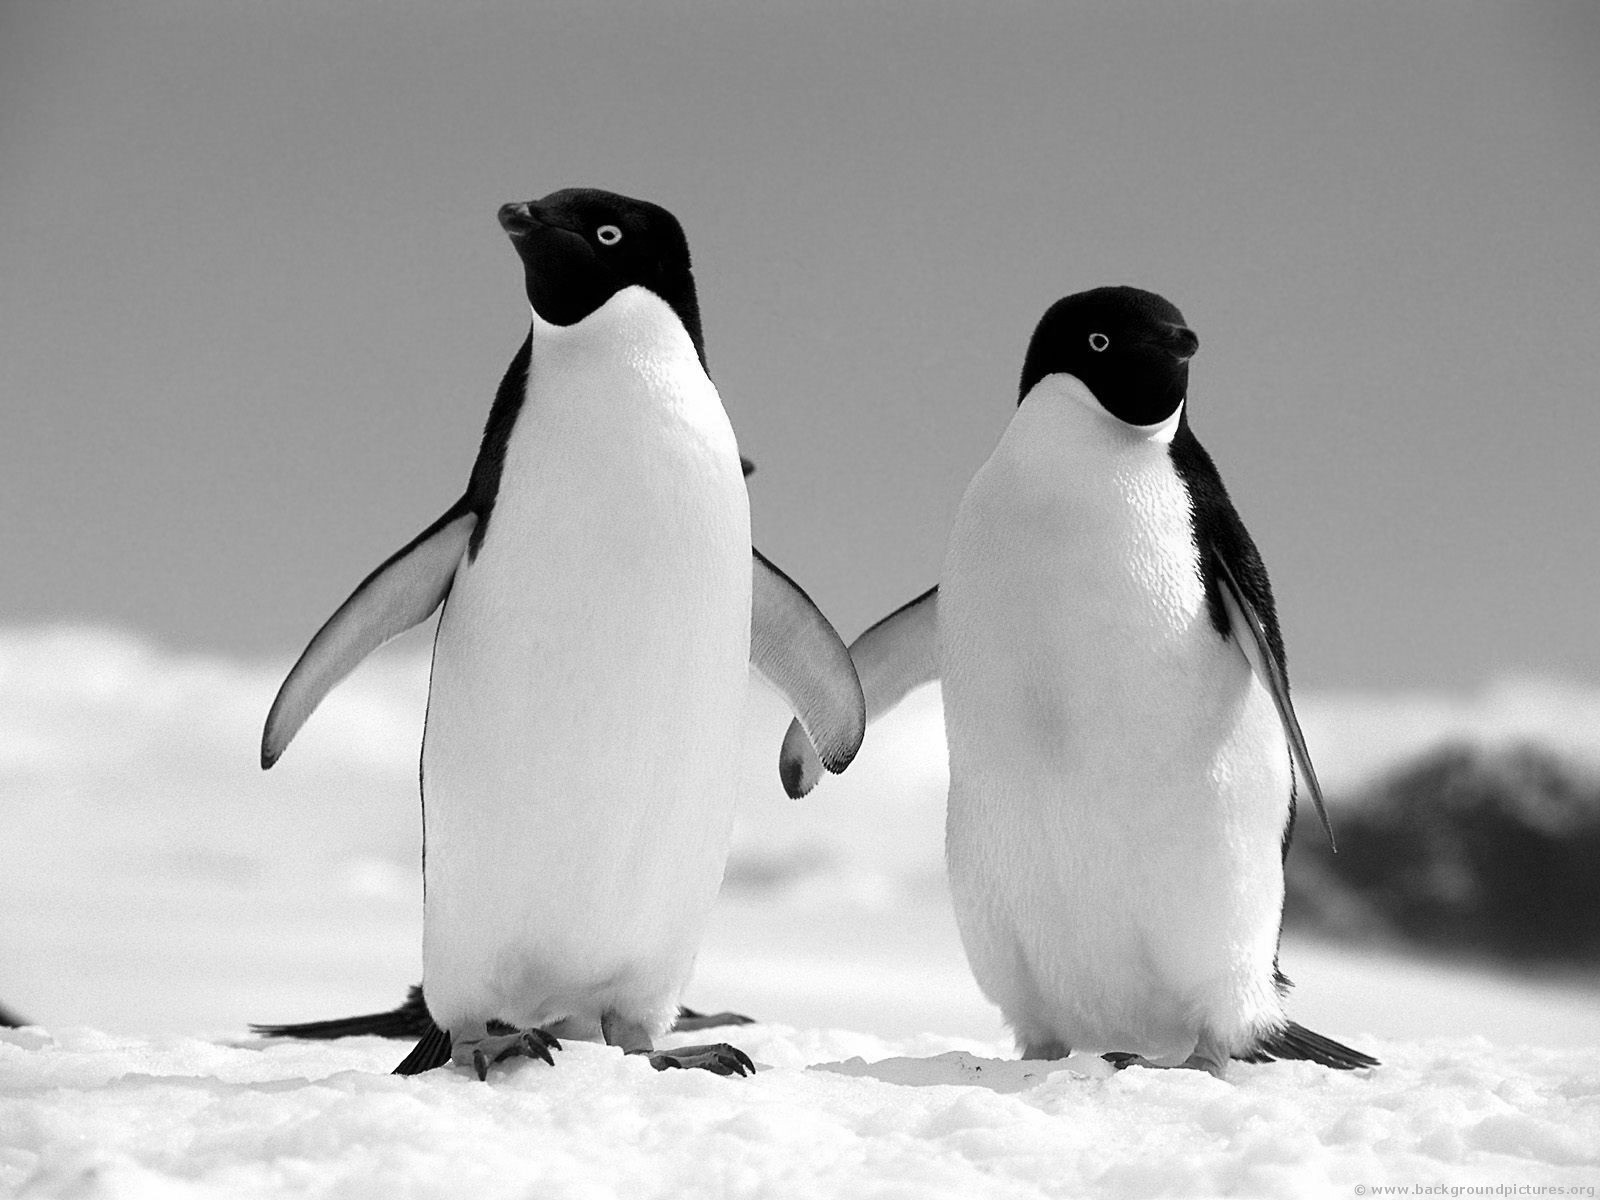
\includegraphics[width=0.9\textwidth]{./kitten-03.jpg}
 % kitten-02.jpg: 1024x768 pixel, 96dpi, 27.09x20.32 cm, bb=0 0 768 576
\end{center} 

\begin{center}\textbf{Thank You!}\end{center}

\end{frame}



\end{document}
